% generated by Docutils <http://docutils.sourceforge.net/>
\documentclass[a4paper,english]{article}
\usepackage{fixltx2e} % LaTeX patches, \textsubscript
\usepackage{cmap} % fix search and cut-and-paste in PDF
\usepackage[T1]{fontenc}
\usepackage[utf8]{inputenc}
\usepackage{ifthen}
\usepackage{babel}
\usepackage{graphicx}
\usepackage{longtable}
\usepackage{array}
\setlength{\extrarowheight}{2pt}
\newlength{\DUtablewidth} % internal use in tables

%%% Custom LaTeX preamble
% PDF Standard Fonts
\usepackage{mathptmx} % Times
\usepackage[scaled=.90]{helvet}
\usepackage{courier}

%%% User specified packages and stylesheets

%%% Fallback definitions for Docutils-specific commands

% hyperlinks:
\ifthenelse{\isundefined{\hypersetup}}{
  \usepackage[unicode,colorlinks=true,linkcolor=blue,urlcolor=blue]{hyperref}
  \urlstyle{same} % normal text font (alternatives: tt, rm, sf)
}{}
\hypersetup{
  pdftitle={Redes de área local},
}

%%% Body
\begin{document}

% Document title
\title{Redes de área local%
  \phantomsection%
  \label{redes-de-area-local}%
  \\ % subtitle%
  \large{Apuntes breves de la materia}%
  \label{apuntes-breves-de-la-materia}}
\author{}
\date{}
\maketitle


%___________________________________________________________________________

\section*{Tema 1: Introducción%
  \phantomsection%
  \addcontentsline{toc}{section}{Tema 1: Introducción}%
  \label{tema-1-introduccion}%
}


%___________________________________________________________________________

\subsection*{0. Aproximación.%
  \phantomsection%
  \addcontentsline{toc}{subsection}{0. Aproximación.}%
  \label{aproximacion}%
}

¿Ventajas de la comunicación instantánea?
%
\begin{itemize}

\item Facilidad de comunicación de ideas.

\item Agilizar trámites

\item Información comercial y bancaria.

\end{itemize}

Un inconveniente de muy alto nivel es el de la privacidad.


%___________________________________________________________________________

\subsection*{1. Características de algunas herramientas%
  \phantomsection%
  \addcontentsline{toc}{subsection}{1. Características de algunas herramientas}%
  \label{caracteristicas-de-algunas-herramientas}%
}


%___________________________________________________________________________

\subsubsection*{1.1 Mensajería instantánea o IM.%
  \phantomsection%
  \addcontentsline{toc}{subsubsection}{1.1 Mensajería instantánea o IM.}%
  \label{mensajeria-instantanea-o-im}%
}
%
\begin{itemize}

\item Instantánea: facilita mucho la comunicación.

\item Proporcionan audio y vídeo.

\item Herramientas gratuitas.

\item Multi-usuario.

\end{itemize}


%___________________________________________________________________________

\subsubsection*{1.2 Blogs (weblog o bitácoras).%
  \phantomsection%
  \addcontentsline{toc}{subsubsection}{1.2 Blogs (weblog o bitácoras).}%
  \label{blogs-weblog-o-bitacoras}%
}
%
\begin{itemize}

\item Alcance universal.

\item Libertad editorial.

\item Anonimato.

\item Suele haber plataformas gratuitas.

\end{itemize}


%___________________________________________________________________________

\subsubsection*{1.3 Podcasts%
  \phantomsection%
  \addcontentsline{toc}{subsubsection}{1.3 Podcasts}%
  \label{podcasts}%
}

Es como un blog sonoro. Consiste simplemente en la difusión de charlas o audio por medio de ficheros de sonido.

Sus ventajas son esencialmente las mismas que las de los blogs.


%___________________________________________________________________________

\subsubsection*{1.4 Wiki%
  \phantomsection%
  \addcontentsline{toc}{subsubsection}{1.4 Wiki}%
  \label{wiki}%
}

Un wiki es una página web modificable por cualquiera (o por casi cualquiera). Al sumar el esfuerzo de muchas personas se puede obtener información muy completa y de muy alta calidad. El inconveniente es que puede haber ``vandalismo''.


%___________________________________________________________________________

\subsubsection*{1.5 Herramientas de aprendizaje.%
  \phantomsection%
  \addcontentsline{toc}{subsubsection}{1.5 Herramientas de aprendizaje.}%
  \label{herramientas-de-aprendizaje}%
}

La enseñanza a distancia se ha visto reforzada y mejorada por las redes de datos. Es mucho más sencillo proporcionar información académica, tutorías, ejercicios, exámenes y demás mediante el uso de ciertos programas.


%___________________________________________________________________________

\subsubsection*{1.6 Cambios en la vida diaria%
  \phantomsection%
  \addcontentsline{toc}{subsubsection}{1.6 Cambios en la vida diaria}%
  \label{cambios-en-la-vida-diaria}%
}
%
\begin{itemize}

\item Pago por tarjeta.

\item Cajeros automáticos

\item Centralitas completas en casa.

\end{itemize}


%___________________________________________________________________________

\subsubsection*{1.7 Ocio%
  \phantomsection%
  \addcontentsline{toc}{subsubsection}{1.7 Ocio}%
  \label{ocio}%
}
%
\begin{itemize}

\item Búsqueda de hoteles/viajes/vuelos...

\item Juegos on-line

\item Chats/Grupos de interés.

\item Vídeo de distribución general

\item Vídeo bajo demanda (Imagenio)

\end{itemize}


%___________________________________________________________________________

\subsection*{2. Función y componentes de redes de datos%
  \phantomsection%
  \addcontentsline{toc}{subsection}{2. Función y componentes de redes de datos}%
  \label{funcion-y-componentes-de-redes-de-datos}%
}


%___________________________________________________________________________

\subsubsection*{2.1 Características básicas%
  \phantomsection%
  \addcontentsline{toc}{subsubsection}{2.1 Características básicas}%
  \label{caracteristicas-basicas}%
}

Que en una hipotética comunicación siempre se debe empezar por tener unas reglas comunes que todo el mundo respeta. A pesar de que se envíe una información nunca hay garantías de que llegue, puede que sea necesario reenviarla.

Además, es muy posible que también haya que tener mecanismos para mejorar la eficiencia de la comunicación.


%___________________________________________________________________________

\subsubsection*{2.2 Funcionamiento%
  \phantomsection%
  \addcontentsline{toc}{subsubsection}{2.2 Funcionamiento}%
  \label{funcionamiento}%
}

Las redes de datos se basan en una jerarquía. Cada miembro de la jerarquía solo conoce un pequeño conjunto de la información total. Al colaborar todas juntas, se consigue el trasiego de información entre puntos muy lejanos.

En esencia, la funcion de las redes es transportar datos de un sitio a otro. Para ello, pueden utilizar mecanismos muy diversos. Sin embargo, casi todos los mecanismos suelen basarse en los mismos principios.


%___________________________________________________________________________

\subsubsection*{2.3 Elementos en redes:%
  \phantomsection%
  \addcontentsline{toc}{subsubsection}{2.3 Elementos en redes:}%
  \label{elementos-en-redes}%
}


%___________________________________________________________________________

\paragraph*{2.3.1 Dispositivos%
  \phantomsection%
  \addcontentsline{toc}{paragraph}{2.3.1 Dispositivos}%
  \label{dispositivos}%
}

Hay dispositivos que no son de uso directo pero son necesarios, como los router.


%___________________________________________________________________________

\paragraph*{2.3.2 Medios%
  \phantomsection%
  \addcontentsline{toc}{paragraph}{2.3.2 Medios}%
  \label{medios}%
}
%
\begin{itemize}

\item Medios inalámbricos: IR, Bluetooth y Wi-Fi

\item Medios alámbricos: Cobre, fibra....

\end{itemize}

Los inalámbricos son más inestables e inseguros pero dan soporte a usuarios móviles. Entre ellos, hay muchas diferencias en cuanto a la capacidad en relación con la distancia.


%___________________________________________________________________________

\paragraph*{2.3.3 Reglas o protocolos.%
  \phantomsection%
  \addcontentsline{toc}{paragraph}{2.3.3 Reglas o protocolos.}%
  \label{reglas-o-protocolos}%
}

Acuerdos establecidos que los fabricantes respetan con el fin de garantizar la interoperabilidad.


%___________________________________________________________________________

\paragraph*{2.3.4 Mensajes%
  \phantomsection%
  \addcontentsline{toc}{paragraph}{2.3.4 Mensajes}%
  \label{mensajes}%
}

Los mensajes en las redes de datos pueden ser convertidos a distintos medios muchas veces, sin embargo todos los dispositivos pueden volver al formato original de forma que se pueda recuperar la información.


%___________________________________________________________________________

\subsubsection*{2.4 Redes convergentes%
  \phantomsection%
  \addcontentsline{toc}{subsubsection}{2.4 Redes convergentes}%
  \label{redes-convergentes}%
}

La tendencia actual es utilizar redes IP para todos los servicios que hay o que pueda haber. Se denomina red convergente a aquella en la que tienen cabida todos los tipos de servicios que se basan en una única infraestructura.


%___________________________________________________________________________

\subsection*{3. Arquitectura de las redes.%
  \phantomsection%
  \addcontentsline{toc}{subsection}{3. Arquitectura de las redes.}%
  \label{arquitectura-de-las-redes}%
}

Las redes informáticas se han construido en base a una serie de principios básicos:


%___________________________________________________________________________

\subsubsection*{3.1. Principios%
  \phantomsection%
  \addcontentsline{toc}{subsubsection}{3.1. Principios}%
  \label{principios}%
}


%___________________________________________________________________________

\paragraph*{3.1.1 Tolerancia a fallas%
  \phantomsection%
  \addcontentsline{toc}{paragraph}{3.1.1 Tolerancia a fallas}%
  \label{tolerancia-a-fallas}%
}

Es la capacidad de la red para recuperarse automáticamente de fallos en determinados puntos de la red.¿Como se consigue?. Por medio de enlaces redundantes que permiten tomar varios caminos a un mismo destino.


%___________________________________________________________________________

\paragraph*{3.1.2 Escalabilidad%
  \phantomsection%
  \addcontentsline{toc}{paragraph}{3.1.2 Escalabilidad}%
  \label{escalabilidad}%
}

Es la capacidad para aumentar de tamaño o prestaciones sin que el conjunto del sistema se vea ralentizado o degradado.¿Como se consigue?. Se consigue haciendo que el diseño no implique el uso de puntos centrales.


%___________________________________________________________________________

\paragraph*{3.1.3 Calidad de servicio%
  \phantomsection%
  \addcontentsline{toc}{paragraph}{3.1.3 Calidad de servicio}%
  \label{calidad-de-servicio}%
}

Es la garantía de que la red ofrece el mejor servicio posible. ¿Como se consigue?. Forzando el uso de protocolos que fomentan la colaboración entre máquinas.


%___________________________________________________________________________

\paragraph*{3.1.4 Seguridad%
  \phantomsection%
  \addcontentsline{toc}{paragraph}{3.1.4 Seguridad}%
  \label{seguridad}%
}

Es la certeza de que la información es procesada solo por quien corresponde.¿Como se consigue?: Mecanismos de cifrado.


%___________________________________________________________________________

\subsubsection*{3.2 Redes basadas en conmutación de paquetes%
  \phantomsection%
  \addcontentsline{toc}{subsubsection}{3.2 Redes basadas en conmutación de paquetes}%
  \label{redes-basadas-en-conmutacion-de-paquetes}%
}

Una red de paquetes se basa en que todo mensaje se trocea. Cada trozo se envía y procesa por separado. Si un paquete se pierde, se reenvía solo ese paquete. Esto permite que:
\newcounter{listcnt0}
\begin{list}{\alph{listcnt0})}
{
\usecounter{listcnt0}
\setlength{\rightmargin}{\leftmargin}
}

\item Si el receptor está ocupado procesando un paquete, el emisor queda libre para enviar otras cosas a otros nodos.

\item Si el emisor falla al enviar un paquete, el receptor no tiene que volver a pedir un archivo completo. Esto mejora mucho la eficiencia.

\item Si algo falla en la red que no sea el emisor ni el receptor, no habrá ningún problema porque se pueden volver a enviar solo los paquetes que se pierdan.

\item Se obtiene una cierta seguridad ya que cada paquete puede viajar por una ruta distinta.
\end{list}


%___________________________________________________________________________

\subsubsection*{3.3 Redes basadas en conmutación de circuitos.%
  \phantomsection%
  \addcontentsline{toc}{subsubsection}{3.3 Redes basadas en conmutación de circuitos.}%
  \label{redes-basadas-en-conmutacion-de-circuitos}%
}

Se basan en que una vez que un usuario inicia una comunicación el cable (o circuito) es para él solo, aunque no lo aproveche al 100\%
\setcounter{listcnt0}{0}
\begin{list}{\alph{listcnt0})}
{
\usecounter{listcnt0}
\setlength{\rightmargin}{\leftmargin}
}

\item Si un emisor o receptor quieren tener garantía absoluta de poder enviar o recibir, se puede alquilar una línea que esté a nuestra disposición todo el tiempo.

\item La eficiencia es mayor que en las redes de paquetes. Aunque todo el mundo esté enviando una línea alquilada pertenece solo a su dueño.
\end{list}


%___________________________________________________________________________

\subsubsection*{3.4 Características específicas de Internet.%
  \phantomsection%
  \addcontentsline{toc}{subsubsection}{3.4 Características específicas de Internet.}%
  \label{caracteristicas-especificas-de-internet}%
}


%___________________________________________________________________________

\paragraph*{3.4.1 Es jerárquica.%
  \phantomsection%
  \addcontentsline{toc}{paragraph}{3.4.1 Es jerárquica.}%
  \label{es-jerarquica}%
}

Significa que hay un orden en cuanto a la organización de los participantes en la red. Este orden suele ser así:
\setcounter{listcnt0}{0}
\begin{list}{\alph{listcnt0})}
{
\usecounter{listcnt0}
\setlength{\rightmargin}{\leftmargin}
}

\item Usuarios: se limitan a consumir y generar datos.

\item ISP: Internet Service Provider o Proveedor de acceso. Son empresas que proporcionan a los usuarios finales los datos necesarios para poder acceder a Internet.

\item Intercambiadores de datos o puntos neutros.

\item Permiten la interconexión de proveedores.
\end{list}


%___________________________________________________________________________

\paragraph*{3.4.2 Estándares comunes%
  \phantomsection%
  \addcontentsline{toc}{paragraph}{3.4.2 Estándares comunes}%
  \label{estandares-comunes}%
}

Un estándar es una norma cuyo cumplimiento ayuda a la interoperabilidad. Los estándares suelen ser gratuitos y cualquiera puede ceñirse a ellos. Los protocolos de Internet son publicos y gratuitos.

El hecho de que los estandares sean comunes ha dado lugar a muchisima competencia y por tanto un mayor desarrollo de Internet.


%___________________________________________________________________________

\paragraph*{3.4.3 Protocolos comunes%
  \phantomsection%
  \addcontentsline{toc}{paragraph}{3.4.3 Protocolos comunes}%
  \label{protocolos-comunes}%
}

El desarrollo de protocolos o estandares es un proceso abierto a la comunidad. CUALQUIERA PUEDE INTENTAR MEJORAR UN PROTOCOLO O HACER UNO NUEVO.

Este mecanismo es muy bueno, porque lo unico que se verifica es que un protocolo sea tecnicamente superior, sin importar de donde viene.


%___________________________________________________________________________

\subsubsection*{3.5 Calidad del servicio%
  \phantomsection%
  \addcontentsline{toc}{subsubsection}{3.5 Calidad del servicio}%
  \label{calidad-del-servicio}%
}

Las redes hoy en dia transportan trafico de muchos tipos. No todo el trafico es tiene los mismos requisitos: existen mecanismos para intentar que todo el mundo obtenga lo que necesite.


%___________________________________________________________________________

\subsection*{3.6 Seguridad%
  \phantomsection%
  \addcontentsline{toc}{subsection}{3.6 Seguridad}%
  \label{id1}%
}

¿Por qué las redes deben ser seguras?.
\setcounter{listcnt0}{0}
\begin{list}{\arabic{listcnt0})}
{
\usecounter{listcnt0}
\setlength{\rightmargin}{\leftmargin}
}

\item Porque por ellas circula información que no debería caer en personas no relacionadas con ella.

\item La información podría ser modificada

\item Se podría modificar la autoría de un mensaje.
\end{list}

Hay otros factores ligados a lo económico. (Phishing). En cualquier caso lograr un cierto grado de seguridad sí es posible. Para ello es muy recomendable utilizar mecanismos de cifrado.


%___________________________________________________________________________

\subsection*{3.7 Integridad en redes.%
  \phantomsection%
  \addcontentsline{toc}{subsection}{3.7 Integridad en redes.}%
  \label{integridad-en-redes}%
}

La integridad es la propiedad que ``garantiza'' que un mensaje no ha sido modificado por error técnico o humano.

En general, para tener la máxima disponibilidad en una red, se suele recurrir a la redundancia, es decir, disponer de más de un mecanismo o dispositivo para que funcione como respaldo del principal.


%___________________________________________________________________________

\subsection*{4. Sistemas de numeración.%
  \phantomsection%
  \addcontentsline{toc}{subsection}{4. Sistemas de numeración.}%
  \label{sistemas-de-numeracion}%
}

Las máquinas digitales utilizan señales eléctricas para la comunicación. El sentido habitual de los términos utilizados es el siguiente
%
\begin{itemize}

\item \textbf{NO HAY PULSO ELÉCTRICO:} Se usa un 0

\item \textbf{SI HAY PULSO ELÉCTRICO:} Se usa un 1

\end{itemize}

Esto da lugar a un problema: las personas utilizan numeración basada en 10 cifras (del 0 al 9). Es necesario establecer mecanismos de conversión


%___________________________________________________________________________

\subsubsection*{4.1 Conversión de decimal a binario%
  \phantomsection%
  \addcontentsline{toc}{subsubsection}{4.1 Conversión de decimal a binario}%
  \label{conversion-de-decimal-a-binario}%
}

Nos dan una cifra como 156 (en base 10) y queremos conocer la representación que hace la máquina (en base 2, en binario)

El procedimiento consiste en ir dividiendo entre dos hasta que no podamos seguir. Despues, se toma el último cociente y todos los restos de final a principio. Esa secuencia de 0 y 1 es el número binario buscado

\leavevmode
\setlength{\DUtablewidth}{\linewidth}
\begin{longtable}[c]{|p{0.110\DUtablewidth}|p{0.203\DUtablewidth}|p{0.168\DUtablewidth}|}
\hline

156:2
 & 
Cociente: 78
 & 
Resto: 0
 \\
\hline

78:2
 & 
Cociente: 39
 & 
Resto: 0
 \\
\hline

39:2
 & 
Cociente: 19
 & 
Resto: 1
 \\
\hline

19:2
 & 
Cociente:  9
 & 
Resto: 1
 \\
\hline

9:2
 & 
Cociente:  4
 & 
Resto: 1
 \\
\hline

4:2
 & 
Cociente:  2
 & 
Resto: 0
 \\
\hline

2:2
 & 
Cociente:  1
 & 
Resto: 0
 \\
\hline
\end{longtable}

Tomamos el último cociente y el último resto y escribimos los restos leyéndolos hacia arriba

10011100 es en binario el número decimal 156

\textbf{Ejercicio} 195 en base decimal necesita ser convertido a binario

195:2   Cociente: 97    Resto: 1
97:2    Cociente: 48    Resto: 1
48:2    Cociente: 24    Resto: 0
24:2    Cociente: 12    Resto: 0
12:2    Cociente:  6    Resto: 0
6:2     Cociente:  3    Resto: 0
3:2     Cociente:  1    Resto: 1

El resultado es 1100.0011

\textbf{Ejercicio} 231 debe pasarse a binario

231:2   Cociente: 115   Resto: 1
115:2   Cociente:  57   Resto: 1
57:2    Cociente:  28   Resto: 1
28:2    Cociente:  14   Resto: 0
14:2    Cociente:   7   Resto: 0
7:2     Cociente:   3   Resto: 1
3:2     Cociente:   1   Resto: 1

La solución es 1110.0111

\textbf{Ejercicio propuesto} 466 debe pasarse a binario (El resultado debe ser 0001.1101.0010)

Hacer las siguientes conversiones
%
\begin{itemize}

\item 567

\item 890

\item 1030

\item 2044

\item 4767 (Solución 1.0010.1001.1111)

\item 6904 (Solución 1.1010.1111.1000)

\end{itemize}


%___________________________________________________________________________

\subsubsection*{4.2 Conversión de binario a decimal%
  \phantomsection%
  \addcontentsline{toc}{subsubsection}{4.2 Conversión de binario a decimal}%
  \label{conversion-de-binario-a-decimal}%
}

Para hacer el proceso inverso debemos escribir las potencias de 2 encima de los bits. Estas potencias se escriben de derecha a izquierda y empezando por 0.

Después se multiplican los bits por las potencias, y estas multiplicaciones se suman. Se debe recordar que algo elevado es 1

Si por ejemplo, nos dan la secuencia 101011, el proceso es el siguiente

\leavevmode
\setlength{\DUtablewidth}{\linewidth}
\begin{longtable}[c]{|p{0.051\DUtablewidth}|p{0.051\DUtablewidth}|p{0.051\DUtablewidth}|p{0.051\DUtablewidth}|p{0.051\DUtablewidth}|p{0.051\DUtablewidth}|}
\hline

2\textasciicircum{}5
 & 
2\textasciicircum{}4
 & 
2\textasciicircum{}3
 & 
2\textasciicircum{}2
 & 
2\textasciicircum{}1
 & 
2\textasciicircum{}0
 \\
\hline

1
 & 
0
 & 
1
 & 
0
 & 
1
 & 
1
 \\
\hline
\end{longtable}

2\textasciicircum{}5 + 2\textasciicircum{}3 + 2\textasciicircum{}1 + 2\textasciicircum{}0 = 32 + 8 + 2 + 1 = 43

Otro ejemplo: Convertir 1001.0011

\leavevmode
\setlength{\DUtablewidth}{\linewidth}
\begin{longtable}[c]{|p{0.051\DUtablewidth}|p{0.051\DUtablewidth}|p{0.051\DUtablewidth}|p{0.051\DUtablewidth}|p{0.051\DUtablewidth}|p{0.051\DUtablewidth}|p{0.051\DUtablewidth}|p{0.051\DUtablewidth}|}
\hline

2\textasciicircum{}7
 & 
2\textasciicircum{}6
 & 
2\textasciicircum{}5
 & 
2\textasciicircum{}4
 & 
2\textasciicircum{}3
 & 
2\textasciicircum{}2
 & 
2\textasciicircum{}1
 & 
2\textasciicircum{}0
 \\
\hline

1
 & 
0
 & 
0
 & 
1
 & 
0
 & 
0
 & 
1
 & 
1
 \\
\hline
\end{longtable}

2\textasciicircum{}7 + 2\textasciicircum{}4 + 2\textasciicircum{}1 + 2\textasciicircum{}0 = 128 + 16 + 2 + 1 = 147


%___________________________________________________________________________

\subsubsection*{4.3 Conversión desde decimal a hexadecimal%
  \phantomsection%
  \addcontentsline{toc}{subsubsection}{4.3 Conversión desde decimal a hexadecimal}%
  \label{conversion-desde-decimal-a-hexadecimal}%
}

El sistema hexadecimal trabaja con 16 símbolos: 0, 1, 2, 3, 4, 5, 6, 7, 8, 9, A, B, C, D, E, F

Se debe tener presente que los símbolos A-F tienen valores internos como estos:
%
\begin{itemize}

\item A = 10

\item B = 11

\item C = 12

\item D = 13

\item E = 14

\item F = 15

\end{itemize}

Para convertir de decimal a hexadecimal debemos dividir por 16 hasta que no se pueda más. Despues se toma el último cociente y todos los restos desde el final hasta el principio.

\textbf{¡CUIDADO!: LOS RESTOS DE LAS DIVISIONES TENDRÁN VALORES COMO 0, 1...7, 8, 9, 10, 11, 12, 13 14 O 15.CUANDO UN RESTO SEA 10, 11, 12, 13, 14 O 15 ESCRIBIREMOS LOS SÍMBOLOS A(10), B(11), C(12), D(13), E(14) O F(15)}

\leavevmode
\setlength{\DUtablewidth}{\linewidth}
\begin{longtable}[c]{|p{0.145\DUtablewidth}|p{0.354\DUtablewidth}|}
\hline

Paso 1
 & 
65535 : 16 4095 y resto 15
 \\
\hline

Paso 2
 & 
495: 16 255 y resto 15
 \\
\hline

Paso 3
 & 
255:16 15 y resto 15
 \\
\hline

Paso 4
 & 
15:16 0 y resto 15
 \\
\hline
\end{longtable}

65535 EN HEXADECIMAL ES FFFF


%___________________________________________________________________________

\subsubsection*{4.4 Conversión desde hexadecimal a decimal%
  \phantomsection%
  \addcontentsline{toc}{subsubsection}{4.4 Conversión desde hexadecimal a decimal}%
  \label{conversion-desde-hexadecimal-a-decimal}%
}

Al igual que antes, se utilizan potencias y sumas. El proceso es exactamente el mismo: se ponen las potencias arriba, de derecha a izquierda, se multiplican y se suman. Sin embargo hay un par de diferencias
\setcounter{listcnt0}{0}
\begin{list}{\arabic{listcnt0})}
{
\usecounter{listcnt0}
\setlength{\rightmargin}{\leftmargin}
}

\item La potencia de base es 16

\item Si encontramos una A, B, C...F debemos utilizar como multiplicador su valor correspondiente.
\end{list}

Ejemplo: Convertir a decimal FFFA

\leavevmode
\setlength{\DUtablewidth}{\linewidth}
\begin{longtable}[c]{|p{0.098\DUtablewidth}|p{0.098\DUtablewidth}|p{0.098\DUtablewidth}|p{0.098\DUtablewidth}|}
\hline

16\textasciicircum{}3
 & 
16\textasciicircum{}2
 & 
16\textasciicircum{}1
 & 
16\textasciicircum{}0
 \\
\hline

F
 & 
F
 & 
F
 & 
A
 \\
\hline
\end{longtable}

Esto es

\leavevmode
\setlength{\DUtablewidth}{\linewidth}
\begin{longtable}[c]{|p{0.110\DUtablewidth}|p{0.517\DUtablewidth}|}
\hline

Paso 1
 & 
F*(16\textasciicircum{}3) + F*(16\textasciicircum{}2) + F*(16\textasciicircum{}1) + A*(16\textasciicircum{}0)
 \\
\hline

Paso 2
 & 
F*(4096) + F*(256) + F*(16) + A*(1)
 \\
\hline

Paso 3
 & 
15*(4096) + 15*(256) + 15*(16) + 10*(1)
 \\
\hline

Paso 4
 & 
61440 + 3840 + 240 + 10= \textbf{65530}
 \\
\hline
\end{longtable}

4.5 Conversión de hexadecimal a binario y viceversa

Para efectuar estas conversiones se necesitan hacer una tabla binaria. Una tabla binaria se construye poniendo 1 y 0 de forma alternativa y en bloques de 0, 1, 2, 4, 8, 16... (en potencias de 2)

\leavevmode
\setlength{\DUtablewidth}{\linewidth}
\begin{longtable}[c]{|p{0.075\DUtablewidth}|p{0.075\DUtablewidth}|p{0.075\DUtablewidth}|p{0.075\DUtablewidth}|p{0.075\DUtablewidth}|}
\hline

0
 & 
0
 & 
0
 & 
0
 & 
0
 \\
\hline

0
 & 
0
 & 
0
 & 
1
 & 
1
 \\
\hline

0
 & 
0
 & 
1
 & 
0
 & 
2
 \\
\hline

0
 & 
0
 & 
1
 & 
1
 & 
3
 \\
\hline

0
 & 
1
 & 
0
 & 
0
 & 
4
 \\
\hline

0
 & 
1
 & 
0
 & 
1
 & 
5
 \\
\hline

0
 & 
1
 & 
1
 & 
0
 & 
6
 \\
\hline

0
 & 
1
 & 
1
 & 
1
 & 
7
 \\
\hline

1
 & 
0
 & 
0
 & 
0
 & 
8
 \\
\hline

1
 & 
0
 & 
0
 & 
1
 & 
9
 \\
\hline

1
 & 
0
 & 
1
 & 
0
 & 
A
 \\
\hline

1
 & 
0
 & 
1
 & 
1
 & 
B
 \\
\hline

1
 & 
1
 & 
0
 & 
0
 & 
C
 \\
\hline

1
 & 
1
 & 
0
 & 
1
 & 
D
 \\
\hline

1
 & 
1
 & 
1
 & 
0
 & 
E
 \\
\hline

1
 & 
1
 & 
1
 & 
1
 & 
F
 \\
\hline
\end{longtable}

Si queremos convertir de hexadecimal a binario el numero C2D7 solo tenemos que convertir elemento a elemento por bloques de 4 bits.

Para convertir desde binario a hexadecimal tenemos que coger los bits de 4 en 4 y empezando por la derecha. Despues cada bloque de 4 bits, se convierte por el elemento de la derecha de la tabla binaria

Por ejemplo, para convertir 1001010010 a hexadecimal tengo que dividir asi: 10.0101.0010. Si un bloque se queda aislado por la izquierda, se pueden añadir ceros para completar hasta 4 bits. El numero binario queda 0010.0101.0010. En informatica, el proceso de rellenar se llama tambien ``padding''.


%___________________________________________________________________________

\paragraph*{Ejercicios%
  \phantomsection%
  \addcontentsline{toc}{paragraph}{Ejercicios}%
  \label{ejercicios}%
}
\setcounter{listcnt0}{0}
\begin{list}{\arabic{listcnt0})}
{
\usecounter{listcnt0}
\setlength{\rightmargin}{\leftmargin}
}

\item De decimal a binario los numeros 46744, 103221

\item De hexadecimal a binario los numeros DE353 y A1B2C3

\item De binario a decimal y hexadecimal 1001.0101.1010.0000 y 1001.1111.0000.1101.1111
\end{list}


%___________________________________________________________________________

\paragraph*{Ejemplo típico de examen%
  \phantomsection%
  \addcontentsline{toc}{paragraph}{Ejemplo típico de examen}%
  \label{ejemplo-tipico-de-examen}%
}

Haz las siguientes conversiones
%
\begin{itemize}

\item 0110010110 a decimal

\item 1875 está en decimal y hay que pasarlo a binario

\item 1875 está en hexadecimal y hay que pasarlo a binario

\item 45509 está de decimal y hay que pasarlo a hexadecimal

\item CADE está en hexadecimal y hay que pasarlo a binario

\end{itemize}


%___________________________________________________________________________

\paragraph*{Solución seleccionada%
  \phantomsection%
  \addcontentsline{toc}{paragraph}{Solución seleccionada}%
  \label{solucion-seleccionada}%
}

01.1001.0110 a decimal
Bits 8 7  4  21

2**8 + 2**7 + 2**4 + 2**2 + 2**1
256  + 128  + 16   + 4    + 2=406


%___________________________________________________________________________

\paragraph*{Solucion seleccionada%
  \phantomsection%
  \addcontentsline{toc}{paragraph}{Solucion seleccionada}%
  \label{id2}%
}

1875 esta en decimal y hay que pasarlo a binario

Lo vamos a convertir primero a hexadecimal
%
\begin{description}
\item[{1875 en hexadecimal es 753 y en binario queda}] \leavevmode 
0111.0101.0011

\end{description}

Solución:

103221 en binario es 0001.1001.0011.0011.0101

\leavevmode
\setlength{\DUtablewidth}{\linewidth}
\begin{longtable}[c]{|p{0.063\DUtablewidth}|p{0.063\DUtablewidth}|p{0.063\DUtablewidth}|p{0.063\DUtablewidth}|p{0.063\DUtablewidth}|p{0.063\DUtablewidth}|}
\hline

A
 & 
1
 & 
B
 & 
2
 & 
C
 & 
3
 \\
\hline

1010
 & 
0001
 & 
1011
 & 
0010
 & 
1100
 & 
0011
 \\
\hline
\end{longtable}


%___________________________________________________________________________

\paragraph*{Solucion seleccionada%
  \phantomsection%
  \addcontentsline{toc}{paragraph}{Solucion seleccionada}%
  \label{id3}%
}

1001.1111.0000.1101.1111 a decimal

Convierto primero a hexadecimal

\leavevmode
\setlength{\DUtablewidth}{\linewidth}
\begin{longtable}[c]{|p{0.063\DUtablewidth}|p{0.063\DUtablewidth}|p{0.063\DUtablewidth}|p{0.063\DUtablewidth}|p{0.063\DUtablewidth}|}
\hline
\multicolumn{5}{|l|}{
1001.1111.0000.1101.1111
} \\
\hline

9
 & 
F
 & 
0
 & 
D
 & 
F
 \\
\hline
\end{longtable}

Y ahora convertimos a decimal
9*16\textasciicircum{}4 + 15*16\textasciicircum{}3 + 13*16\textasciicircum{}1 + 15*16\textasciicircum{}0 = 651487


%___________________________________________________________________________

\subsection*{5 Estructura general de una red.%
  \phantomsection%
  \addcontentsline{toc}{subsection}{5 Estructura general de una red.}%
  \label{estructura-general-de-una-red}%
}

Toda red tiene un conjunto de elementos que interoperan entre ellos.

Supongamos que una máquina con XP desea enviar un mensaje como ``Hola'' a través de Internet a una máquina que usa Linux.
%
\begin{itemize}

\item Origen: es la máquina que envía el mensaje.

\item Codificación: La A en el origen se representa con un binario, como por ejemplo 1000.0001

\item Transmisor: Por ejemplo, un router basado en cable.

\item Medio: Elemento pasivo por el cual circulan los mensajes.

\item Receptor: Por ejemplo, un router inalámbrico.

\item Descodificación: Se recoge el 1000.0001 y se convierte (por ejemplo erróneamente) a ``ú''

\item Destinatario: La máquina que recibe el mensaje (en este caso ``ú''

\end{itemize}

En general, en cualquier red informática la información se envía troceada. Este troceado se denomina ``segmentación''.

Al trocear la información podemos ``compartir'' líneas de forma que cada uno la utilice ``un poco''. Este compartición se denomina multiplexación. Para que todo funcione correctamente es imprescindible que cada trozo o segmento lleve una numeración o marca que lo identifique y que permita al receptor reconstruir el mensaje inicial.


%___________________________________________________________________________

\subsubsection*{5.1 Componentes de una red%
  \phantomsection%
  \addcontentsline{toc}{subsubsection}{5.1 Componentes de una red}%
  \label{componentes-de-una-red}%
}


%___________________________________________________________________________

\paragraph*{5.1.1 Componentes hardware%
  \phantomsection%
  \addcontentsline{toc}{paragraph}{5.1.1 Componentes hardware}%
  \label{componentes-hardware}%
}

Son los elementos físicos que intervienen en la comunicación: router, módem, switches, proxies....


%___________________________________________________________________________

\paragraph*{5.1.2 Componentes software%
  \phantomsection%
  \addcontentsline{toc}{paragraph}{5.1.2 Componentes software}%
  \label{componentes-software}%
}

Son programas que se ejecutan en un hardware con el fin de ofrecer un servicio. Ej: DNS, TCP/IP

En los componentes software, no todos los elementos actúan de la misma manera.
%
\begin{itemize}

\item Clientes: un programa que solicita una tarea directamente relacionada con el usuario final.

\item Servidores: no interactúan el usuario, sino con programas clientes.

\item A veces, hay programas que pueden hacer las dos tareas a la vez, aunque no son tan frecuentes.

\end{itemize}


%___________________________________________________________________________

\subsubsection*{5.2 Intermediarios.%
  \phantomsection%
  \addcontentsline{toc}{subsubsection}{5.2 Intermediarios.}%
  \label{intermediarios}%
}

Se denomina dispositivos intermediarios a todos aquellos que no están bajo nuestro control pero que efectúan tareas de encaminamiento de la información.

Se puede usar el comando tracert www.google.com (o cualquier otro sitio) para verificar si un problema está en nuestra red o no.

Estos dispositivos intermediarios pueden tomar decisiones en cuanto a los caminos más apropiados para enviar un segmento a su destino. También son capaces de solicitar retransmisiones y detectar errores.


%___________________________________________________________________________

\subsubsection*{5.3 Medios%
  \phantomsection%
  \addcontentsline{toc}{subsubsection}{5.3 Medios}%
  \label{id4}%
}

Los medios, que eran elementos pasivos, se pueden clasificar en tres grandes tipos.
\setcounter{listcnt0}{0}
\begin{list}{\arabic{listcnt0})}
{
\usecounter{listcnt0}
\setlength{\rightmargin}{\leftmargin}
}

\item Cobre

\item Fibra óptica

\item Pulsos EM.
\end{list}


%___________________________________________________________________________

\paragraph*{5.3.1 Cobre%
  \phantomsection%
  \addcontentsline{toc}{paragraph}{5.3.1 Cobre}%
  \label{cobre}%
}

El cobre es un ``relativamente bueno'' conductor de electricidad. Así, podemos enviar 1 y 0's a lo largo de un cable de cobre por medio de impulsos eléctricos.


%___________________________________________________________________________

\paragraph*{5.3.2 Fibra óptica%
  \phantomsection%
  \addcontentsline{toc}{paragraph}{5.3.2 Fibra óptica}%
  \label{fibra-optica}%
}

Se basa en conducir impulsos lumínicos. Debido a que la luz es el elemento más rápido conocido la velocidad que alcanzan estos cables suele ser mucho mayor. El problema de la fibra es el coste.

Hay dos formas de usar fibra:
%
\begin{itemize}

\item Monomodo: el rayo de luz avanza en línea recta. Más rápido, pero se requiere una luz más intensa (láser).

\item Multimodo: permite que varios rayos de luz crucen el cable. Se puede usar un diodo LED normal.

\end{itemize}


%___________________________________________________________________________

\paragraph*{5.3.3 Electromagnetismo%
  \phantomsection%
  \addcontentsline{toc}{paragraph}{5.3.3 Electromagnetismo}%
  \label{electromagnetismo}%
}

El estándar más popular es Wi-Fi. Permite una comodidad mayor para el usuario. El problema de las redes inalámbricas es doble: la seguridad y el otro la variabilidad de la señal.


%___________________________________________________________________________

\paragraph*{5.3.4 Consideraciones generales%
  \phantomsection%
  \addcontentsline{toc}{paragraph}{5.3.4 Consideraciones generales}%
  \label{consideraciones-generales}%
}

A la hora de elegir un medio para nuestra red se deben tener en cuenta estos tres factores
%
\begin{itemize}

\item Ancho de banda

\item Coste

\item Entorno (movilidad o no, industriales)

\end{itemize}


%___________________________________________________________________________

\subsubsection*{5.4 Tipos de red%
  \phantomsection%
  \addcontentsline{toc}{subsubsection}{5.4 Tipos de red}%
  \label{tipos-de-red}%
}


%___________________________________________________________________________

\paragraph*{5.4.1 Red local o LAN (Local Area Network)%
  \phantomsection%
  \addcontentsline{toc}{paragraph}{5.4.1 Red local o LAN (Local Area Network)}%
  \label{red-local-o-lan-local-area-network}%
}

Es una red de alcance pequeño: una sala o un edificio.


%___________________________________________________________________________

\paragraph*{5.4.2 Red metropolitana o MAN (Metropolitan AN)%
  \phantomsection%
  \addcontentsline{toc}{paragraph}{5.4.2 Red metropolitana o MAN (Metropolitan AN)}%
  \label{red-metropolitana-o-man-metropolitan-an}%
}

Un barrio o una ciudad


%___________________________________________________________________________

\paragraph*{5.4.3 Redes de area amplia o WAN (Wide AN)%
  \phantomsection%
  \addcontentsline{toc}{paragraph}{5.4.3 Redes de area amplia o WAN (Wide AN)}%
  \label{redes-de-area-amplia-o-wan-wide-an}%
}

Cubren áreas geográficas muy grandes: países e incluso continentes. Los proveedores de servicios internet o Internet Service Providers son los únicos que implantan redes de área amplia. Con ello, ofrecen sus servicios a usuario locales que desean estar interconectados con otros usuario.


%___________________________________________________________________________

\subsubsection*{5.5 Internet%
  \phantomsection%
  \addcontentsline{toc}{subsubsection}{5.5 Internet}%
  \label{internet}%
}

Internet es el resultado de interconectar redes aisladas. El hardware necesario lo proporcionan las compañías de teléfono. El software de IP ES GRATIS.

En Internet cada uno puede hacer lo que quiera DENTRO DE SU LAN. La conexion al exterior de esa LAN es del proveedor. En ese punto ``fronterizo'' se deben respetar todos los estándares. El hecho de que sea el software el principal ``pegamento'' de distintas redes es lo que permite que un usuario con conexión inalámbrica se conecte con uno que usa ADSL en otro punto del mundo cruzando distintos tipos de línea.


%___________________________________________________________________________

\subsubsection*{5.6 Intranet%
  \phantomsection%
  \addcontentsline{toc}{subsubsection}{5.6 Intranet}%
  \label{intranet}%
}

Es una red privada de una compañía que usa Internet. Normalmente, para ver documentos o archivos de esa empresa será necesario un usuario y una contraseña.


%___________________________________________________________________________

\subsection*{6 Protocolos%
  \phantomsection%
  \addcontentsline{toc}{subsection}{6 Protocolos}%
  \label{protocolos}%
}

Un protocolo es un conjunto de reglas que hay que respetar para conseguir que la comunicación funcione.

Los protocolos de red necesitan poner de acuerdo a las máquinas en cosas como:
%
\begin{itemize}

\item Formato: p.ej ¿qué tamaño de segmento se usará?

\item Proceso: p.ej forzando a las máquinas a colaborar

\item Errores: unificando los códigos de error.

\item Terminación: determinando como se debe terminar.

\end{itemize}


%___________________________________________________________________________

\subsection*{7. Conjuntos de protocolos%
  \phantomsection%
  \addcontentsline{toc}{subsection}{7. Conjuntos de protocolos}%
  \label{conjuntos-de-protocolos}%
}

A menudo, los protocolos no se han diseñado de forma aislada. Es más frecuente que los protocolos se diseñen e implementen como un conjunto. Por ejemplo, TCP/IP son solo dos protocolos de una familia.

Hay dos grandes familias de protocolos: OSI y TCP/IP

En una familia de protocolos hay distintas funciones. Esto se debe a que la comunicación es una tarea MUY compleja. Para hacerlo más sencillo, se divide la tarea en subtareas.


%___________________________________________________________________________

\subsubsection*{7.1 OSI%
  \phantomsection%
  \addcontentsline{toc}{subsubsection}{7.1 OSI}%
  \label{osi}%
}

En OSI los protocolos se organizan en ``capas''. La idea subyacente es que podamos cambiar capas fácilmente. En OSI hay 7 capas.

\leavevmode
\setlength{\DUtablewidth}{\linewidth}
\begin{longtable}[c]{|p{0.377\DUtablewidth}|}
\hline

Aplicación
 \\
\hline

Presentación
 \\
\hline

Sesión
 \\
\hline

Transporte
 \\
\hline

Red
 \\
\hline

Enlace
 \\
\hline

Física
 \\
\hline
\end{longtable}


%___________________________________________________________________________

\paragraph*{7.1.1 Física%
  \phantomsection%
  \addcontentsline{toc}{paragraph}{7.1.1 Física}%
  \label{fisica}%
}

Se encarga de las normas sobre forma de los conectores, voltajes en los cables


%___________________________________________________________________________

\paragraph*{7.1.2 Enlace%
  \phantomsection%
  \addcontentsline{toc}{paragraph}{7.1.2 Enlace}%
  \label{enlace}%
}

Se encarga de regular los envíos de datos entre vecinos inmediatos. Por ejemplo, en las redes locales Ethernet el enlace utiliza segmentos de 1500 bytes. Otro ejemplo es que en la capa de enlace se pueden enviar datos y despues el receptor debe CONFIRMARNOs de alguna forma que los datos llegan.


%___________________________________________________________________________

\paragraph*{7.1.3 Red%
  \phantomsection%
  \addcontentsline{toc}{paragraph}{7.1.3 Red}%
  \label{red}%
}

Regula la transmisión entre vecinos lejanos. Un ejemplo de elemento regulado son las direcciones que todo el mundo debe tener.


%___________________________________________________________________________

\paragraph*{7.1.4 Transporte%
  \phantomsection%
  \addcontentsline{toc}{paragraph}{7.1.4 Transporte}%
  \label{transporte}%
}

Se ocupa de que una misma conexión se pueda usar por muchos programas en el mismo ordenador. La capa de transporte permite multiplexar el cable por medio de una numeración especial que llamamos ``puertos''.


%___________________________________________________________________________

\paragraph*{7.1.5 Sesión%
  \phantomsection%
  \addcontentsline{toc}{paragraph}{7.1.5 Sesión}%
  \label{sesion}%
}

Regula los procedimientos para iniciar y cerrar conexiones: uso de contraseñas, cifrados, tarificación.


%___________________________________________________________________________

\paragraph*{7.1.6 Presentación%
  \phantomsection%
  \addcontentsline{toc}{paragraph}{7.1.6 Presentación}%
  \label{presentacion}%
}

Que regula cosas como ¿qué número se va a utilizar para representar cada letra?. Por ejemplo, la A usará el código 65


%___________________________________________________________________________

\paragraph*{7.1.7 Aplicación%
  \phantomsection%
  \addcontentsline{toc}{paragraph}{7.1.7 Aplicación}%
  \label{aplicacion}%
}

Son los programas que utiliza el usuario final. Se regulan cosas como intercambio de archivos, de páginas HTML


%___________________________________________________________________________

\subsubsection*{7.2 TCP/IP%
  \phantomsection%
  \addcontentsline{toc}{subsubsection}{7.2 TCP/IP}%
  \label{tcp-ip}%
}

Es más sencillo. Elimina diversas capas y triunfó gracias a que funcionó desde el primer momento y a que era gratuito.

\leavevmode
\setlength{\DUtablewidth}{\linewidth}
\begin{longtable}[c]{|p{0.377\DUtablewidth}|}
\hline

Aplicación
 \\
\hline

Transporte
 \\
\hline

Interred
 \\
\hline

Física
 \\
\hline
\end{longtable}


%___________________________________________________________________________

\paragraph*{7.2.1 Física%
  \phantomsection%
  \addcontentsline{toc}{paragraph}{7.2.1 Física}%
  \label{id5}%
}

TCP/IP NO REGULA NADA DE CAPA FÍSICA


%___________________________________________________________________________

\paragraph*{7.2.2 Interred%
  \phantomsection%
  \addcontentsline{toc}{paragraph}{7.2.2 Interred}%
  \label{interred}%
}

Es una mezcla de la de red y enlace OSI. El protocolo más usado es IP


%___________________________________________________________________________

\paragraph*{7.2.3 Transporte%
  \phantomsection%
  \addcontentsline{toc}{paragraph}{7.2.3 Transporte}%
  \label{id6}%
}

El protocolo más usado es TCP y despues UDP. Se encarga de lo mismo que la de transporte OSI.


%___________________________________________________________________________

\paragraph*{7.2.4 Aplicación%
  \phantomsection%
  \addcontentsline{toc}{paragraph}{7.2.4 Aplicación}%
  \label{id7}%
}

Dan libertad a los programadores de aplicaciones para que creen sus propios protocolos.


%___________________________________________________________________________

\subsubsection*{7.3 Independencia de la tecnología%
  \phantomsection%
  \addcontentsline{toc}{subsubsection}{7.3 Independencia de la tecnología}%
  \label{independencia-de-la-tecnologia}%
}

Los protocolos en las redes son independientes del tipo de medio físico, cable, pulso EM o lo que sea. Es así porque si en el futuro aparecen tecnologías nuevas podría ocurrir que los protocolos quedasen obsoletos junto a los viejos ``cables''.


%___________________________________________________________________________

\subsection*{8. Consideraciones en los modelos de capas%
  \phantomsection%
  \addcontentsline{toc}{subsection}{8. Consideraciones en los modelos de capas}%
  \label{consideraciones-en-los-modelos-de-capas}%
}

Los modelos basados en capas son muy populares, pero ¿por qué diseñar software basándonos en esta arquitectura?. Hay varias razones
%
\begin{itemize}

\item Es más fácil diseñar algo al poder trocear las partes y ocuparnos cada uno de una parte.

\item Fomentar la competencia haciendo que muchos fabricantes ofrecieran distintas versiones de los mismos protocolos haciendo que el precio bajara y la calidad subiera.

\item Se pretendía que fuera fácil sustituir unos protocolos por otros. Esto facilita la vida de los usuarios.

\item Se pretendía tener un conjunto de términos comunes para definir todos los conceptos.

\end{itemize}


%___________________________________________________________________________

\subsubsection*{8.1 Encapsulación%
  \phantomsection%
  \addcontentsline{toc}{subsubsection}{8.1 Encapsulación}%
  \label{encapsulacion}%
}

Encapsulación es el proceso por el cual las capas cogen datos de sus capas vecinas SIN MIRAR PARA NADA LO QUE HAY. Procesan dichos datos y añaden la información necesaria para los destinatarios. La idea es tratar la información que llega como una cápsula que no podemos abrir ni tocar.

En relación con esto se definen distintas PDU. Una PDU es una ``Protocol Data Unit'' o ``Unidad de datos de protocolo''. Cada capa recibe una PDU (o bloque), la toma, le añade lo que sea necesaria y eso se convierte una PDU nueva que se pasa hacia abajo. Los distintos nombres de las PDU son estos
%
\begin{itemize}

\item Trama: Bloque de capa de enlace.

\item Datagrama: Bloque de capa de red.

\item Segmento: Bloque de capa de transporte.

\item Paquete: Capa de aplicación.

\end{itemize}

Cada PDU tiene su propia información especial: por ejemplo los segmentos necesitan los números de puerto, los datagramas necesitan las IP de origen y destino.


%___________________________________________________________________________

\subsubsection*{8.2 Direccionamiento%
  \phantomsection%
  \addcontentsline{toc}{subsubsection}{8.2 Direccionamiento}%
  \label{direccionamiento}%
}

Cada capa puede tener su propia dirección especial. Es importante recalcar que las direcciones NO VAN ASOCIADAS A LOS EQUIPOS, sino a SUS CONEXIONES. Por tanto, si un equipo tiene varias tarjetas, podría tener varias direcciones.

Algunos ejemplo de direcciones serían los siguientes
%
\begin{itemize}

\item Dirección DNS:        www.google.com (1024 caract)

\item Dirección de TCP:     Puerto 80 (16 bits)

\item Dirección IP:         66.249.92.104 (32 bits)

\item Dirección Ethernet:   01:DC:43:23:99:7B (48 bits)

\end{itemize}


%___________________________________________________________________________

\section*{Tema 2: Nivel físico%
  \phantomsection%
  \addcontentsline{toc}{section}{Tema 2: Nivel físico}%
  \label{tema-2-nivel-fisico}%
}


%___________________________________________________________________________

\subsection*{0. Introducción%
  \phantomsection%
  \addcontentsline{toc}{subsection}{0. Introducción}%
  \label{introduccion}%
}

Es la única capa que no es software sino elementos físicos. En general tenemos tres grandes categorías de medios físicos
\setcounter{listcnt0}{0}
\begin{list}{\arabic{listcnt0})}
{
\usecounter{listcnt0}
\setlength{\rightmargin}{\leftmargin}
}

\item Cobre

\item Fibra

\item Pulsos EM.
\end{list}


%___________________________________________________________________________

\subsection*{1. Función%
  \phantomsection%
  \addcontentsline{toc}{subsection}{1. Función}%
  \label{funcion}%
}

La capa física se encarga de transportar bits convirtiéndolos primero al tipo de señal correspondiente al medio físico y luego extrae de esos medios físicos los bits.

Esta tarea requiere de varios elementos:
\setcounter{listcnt0}{0}
\begin{list}{\alph{listcnt0})}
{
\usecounter{listcnt0}
\setlength{\rightmargin}{\leftmargin}
}

\item Medio físico

\item Mecanismo de representación (p. ej 0V->bit 0, 5V->1)

\item Circuitería electrónica: esto supone que habrá un coste.

\item Mecanismos de codificación (p. ej, asignación de bloques).
\end{list}

Se llama señalización al proceso de conversión de una secuencia de bits en una secuencia de impulsos.


%___________________________________________________________________________

\subsubsection*{1.1 Modulación/demodulación.%
  \phantomsection%
  \addcontentsline{toc}{subsubsection}{1.1 Modulación/demodulación.}%
  \label{modulacion-demodulacion}%
}

Se llama modulación al proceso de modificación de una señal para que transporte bits. Toda señal tiene una amplitud y una frecuencia. Se llama Amplitud al punto más alto (o bajo) de una señal. Se llama frecuencia al número de ondas completas que transcurren en un segundo.

Tanto la amplitud como la frecuencia se pueden modular lo que nos lleva a los dos procesos fundamentales de modulación: AM y FM


%___________________________________________________________________________

\paragraph*{1.1.1 Modulacion AM%
  \phantomsection%
  \addcontentsline{toc}{paragraph}{1.1.1 Modulacion AM}%
  \label{modulacion-am}%
}

La modulación en amplitud permite alcances mucho mayores y se basa en la alteración de la amplitud o altura de la señal

Utilizando lápiz y papel dibuja la señal generada utilizando un esquema de modulacion AM de 4 señales que envíe la cadena de bits 0111.0010

Solucion

\noindent\makebox[\textwidth][c]{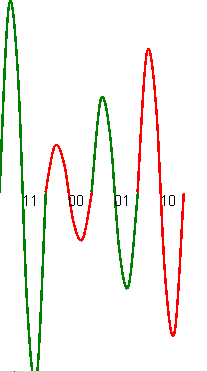
\includegraphics[scale=0.650000]{img/t2/ModulacionAM.png}}

La creación de señales tiene una serie de principios básicos:
\setcounter{listcnt0}{0}
\begin{list}{\alph{listcnt0})}
{
\usecounter{listcnt0}
\setlength{\rightmargin}{\leftmargin}
}

\item Todos los tiempos son iguales: todos los intervalos de tiempo deben ser igual de anchos.

\item Si me dicen que hay 4 niveles, es porque se van a enviar bits de 4 en 4. Se deben crear todas las combinaciones de 4 (desde 0000, 0001....1111)

\item Toda señal debe alcanzar la máxima y mínima altura por encima y por debajo del eje de las X.

\item Debemos escribir todas las combinaciones por arriba y por debajo del eje de las X

\item Divido la cadena en bloques de 4. Si me hace falta añado ceros por la izquierda.
\end{list}


%___________________________________________________________________________

\paragraph*{Para practicar en casa%
  \phantomsection%
  \addcontentsline{toc}{paragraph}{Para practicar en casa}%
  \label{para-practicar-en-casa}%
}

Utilizando un esquema de 2 bits enviar la cadena 00100101

Utilizando un esquema de 3 bits enviar la cadena 101001011

Utilizando un esquema de 4 bits enviar la cadena 0010010101101


%___________________________________________________________________________

\paragraph*{1.1.2 Modulación FM%
  \phantomsection%
  \addcontentsline{toc}{paragraph}{1.1.2 Modulación FM}%
  \label{modulacion-fm}%
}

La modulación FM es un mecanismo basado en modificar el número de ondas por tiempo.

Solo hay que elegir un esquema de codificación basándonos en el número de ondas. P.ej:
%
\begin{itemize}

\item 000-{}-{}->1 onda

\item 001-{}-{}->2 ondas

\item 010-{}-{}->3 ondas

\item 011-{}-{}->4 ondas

\item 100-{}-{}->5 ondas

\item 101-{}-{}->6 ondas

\item 110-{}-{}->7 ondas

\item 111-{}-{}->8 ondas

\end{itemize}

\noindent\makebox[\textwidth][c]{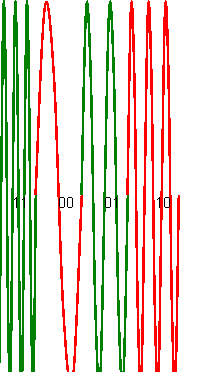
\includegraphics[scale=0.650000]{img/t2/ModulacionFM.png}}


%___________________________________________________________________________

\paragraph*{1.1.3 Modulación PM/PSK o modulación de fase.%
  \phantomsection%
  \addcontentsline{toc}{paragraph}{1.1.3 Modulación PM/PSK o modulación de fase.}%
  \label{modulacion-pm-psk-o-modulacion-de-fase}%
}

La modulación en fase se basa en modificar el punto en el que empieza una onda. Al final, todas las ondas empiezan y acaban en el mismo punto y además todas pasan por el punto más alto y por el punto más bajo.

Se debe tener en cuenta que en todos los mecanismos de modulación se cumple la misma regla:\emph{``Cuantos más estados de modulación (divisiones) más bits por onda y por tanto más velocidad. Sin embargo, las señales se vuelven mucho más complicadas de entender y de generar''} Esto se ilustra en la imagen donde se ven la emisión de bits. Es estas emisiones pueden meterse muchos bits por onda, o muy pocos.

\noindent\makebox[\textwidth][c]{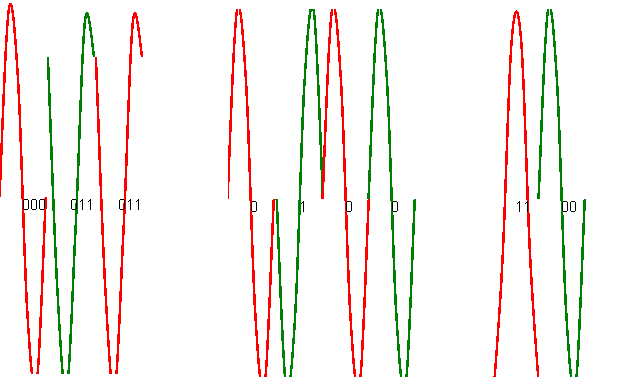
\includegraphics[scale=0.450000]{img/t2/TresModulacionesPM.png}}

Dibujar las fases y comprender como funcionan puede ser complejo. Para facilitarlo se muestran en la figura siguiente unas ilustraciones explicativas en las que se pueden ver como el ángulo de ``desfase'' marca el punto donde la onda empezará y terminará así como si empezará subiendo o bajando. Mirando los dibujos de derecha a izquierda y de arriba a abajo se pueden ver las ondas con desfases de 0, 45, 90, 135, 180, 215, 270 y 315 grados. Como se puede apreciar, este esquema, al utilizar 8 ondas posibles puede enviar grupos de 3 bits de una sola vez. Si se desearan enviar grupos de 4 bits por onda habría que ``dividir'' el círculo en 16 fases utilizar cada una de ellas para enviar 0000, 0001, 0010, 0011, ..., 1110 y 1111

\noindent\makebox[\textwidth][c]{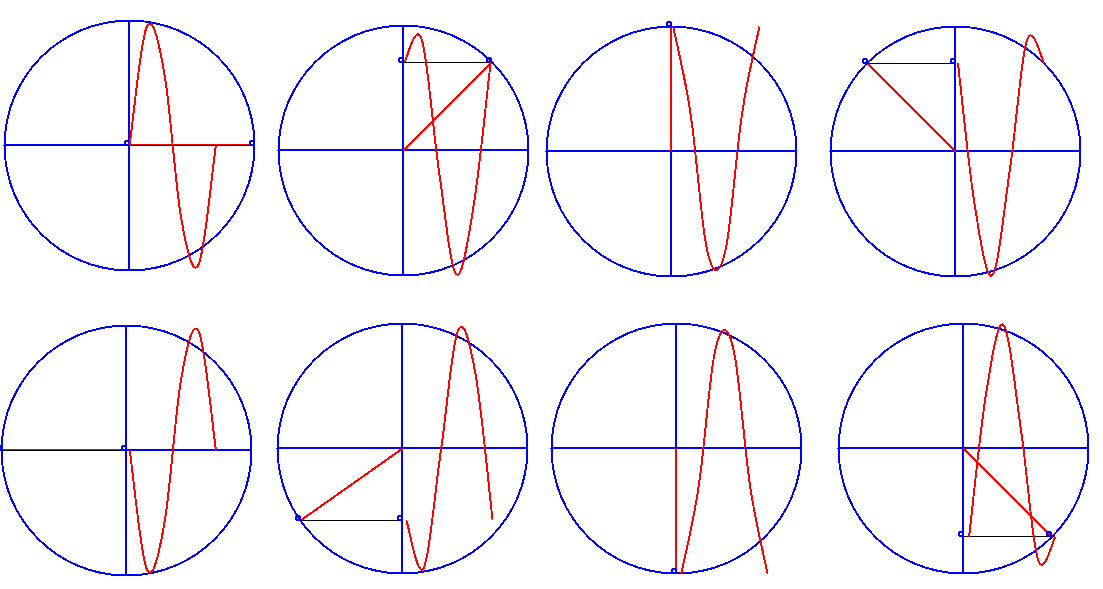
\includegraphics[width=0.800\linewidth]{img/t2/EsquemaFases.png}}


%___________________________________________________________________________

\paragraph*{1.1.4 Sistemas mixtos.%
  \phantomsection%
  \addcontentsline{toc}{paragraph}{1.1.4 Sistemas mixtos.}%
  \label{sistemas-mixtos}%
}

En la vida real, es muy extraño encontrar dispositivos que solo usen AM, FM o PM. Lo más normal es que se combinen varios mecanismos para intentar aprovechar las ventajas de cada uno ellos.De hecho, se pueden combinar los tres sistemas a la vez mezclando modulación de frecuencias, fases y amplitudes

En un sistema que combinara 2 niveles de AM con dos de FM tendríamos cuatro posibles formas de onda
%
\begin{itemize}

\item Onda 00: Amplitud 1 y Frecuencia 1

\item Onda 01: Amplitud 1 y Frecuencia 2

\item Onda 10: Amplitud 2 y Frecuencia 1

\item Onda 11: Amplitud 2 y Frecuencia 2

\end{itemize}

\noindent\makebox[\textwidth][c]{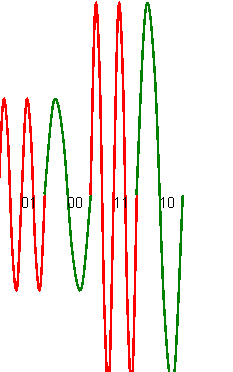
\includegraphics[width=0.450\linewidth]{img/t2/ModulacionAM_y_FM.png}}


%___________________________________________________________________________

\subparagraph*{Ejercicio%
  \phantomsection%
  \addcontentsline{toc}{subparagraph}{Ejercicio}%
  \label{ejercicio}%
}

Para el próximo día se propone crear el esquema que combina 4 fases, 2 frecuencias, 4 alturas.


%___________________________________________________________________________

\subsection*{2. Transmisión/recepción en analógico o digital.%
  \phantomsection%
  \addcontentsline{toc}{subsection}{2. Transmisión/recepción en analógico o digital.}%
  \label{transmision-recepcion-en-analogico-o-digital}%
}

Se dice que una señal es analógica cuando se acepta que tome cualquier valor en un intervalo dado. Una señal es digital cuando solo se aceptan ciertos valores de la señal. La señal digital más básica es aquella que solo utiliza dos niveles correspondientes a los bits 0 y 1.

Las señales analógicas emitidas no pueden ser procesadas ``demasiado bien'' por el receptor, ya que al fin y al cabo pueden ocurrir muchas cosas que alteren la señal de forma que el receptor no pueda saber la forma original de la señal

Sin embargo, las señales digitales pueden ser procesadas por el receptor y reconstruidas al saber que no todo es posible, por lo tanto la señal original se puede reconstruir ``casi'' a la perfección. Aún así se debe tener en cuenta que \emph{cuando una señal analógica se convierte a digital se pierde información.} La imagen siguiente muestra como una señal analógica original se ha muestreado utilizando menos o más bits de forma que la señal digitalizada puede ser menos o más fiel a la original. Sin embargo, más fidelidad requiere más memoria.

\noindent\makebox[\textwidth][c]{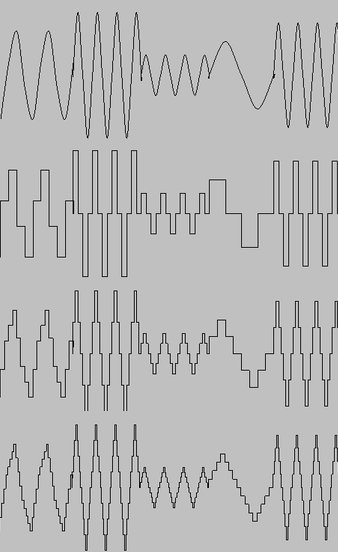
\includegraphics[width=0.450\linewidth]{img/t2/Muestreo.png}}


%___________________________________________________________________________

\subsection*{3. Transmisión o recepción síncrona/asíncrona.%
  \phantomsection%
  \addcontentsline{toc}{subsection}{3. Transmisión o recepción síncrona/asíncrona.}%
  \label{transmision-o-recepcion-sincrona-asincrona}%
}

Cuando alguien envía una señal digital, surge un problema importante. ¿Donde empieza y acaba un bit?.

Para resolver este problema hay dos soluciones:
\setcounter{listcnt0}{0}
\begin{list}{\alph{listcnt0})}
{
\usecounter{listcnt0}
\setlength{\rightmargin}{\leftmargin}
}

\item Transmisión síncrona: el emisor envía una señal junto a la señal de datos que marca los comienzos y los finales. Es decir, que nos envía dos cosas a la vez, la señal de sincronismo y la de datos.

\item Transmisión asíncrona: solo nos envía una cosa. Primero se envía una señal por delante que sean unos y ceros consecutivos. Esta señal le sirve al receptor para saber como de largos son los pulsos. Despues, el emisor envía datos, y el receptor ya sabe como de largos son los bits y sabe ``por donde cortar''.
\end{list}


%___________________________________________________________________________

\subsection*{4. Transmisión en serie o en paralelo%
  \phantomsection%
  \addcontentsline{toc}{subsection}{4. Transmisión en serie o en paralelo}%
  \label{transmision-en-serie-o-en-paralelo}%
}

Una transmisión en serie es una transmisión/recepción que solo utiliza un cable. Los datos se envían uno tras otro. Se ahorra cobre pero la velocidad es más pequeña.

Una transmisión en paralelo utiliza muchos cables a la vez para enviar muchos bits a la vez. Se utiliza más cobre pero la velocidad se multiplica.


%___________________________________________________________________________

\subsection*{5. Codificaciones/Descodificaciones%
  \phantomsection%
  \addcontentsline{toc}{subsection}{5. Codificaciones/Descodificaciones}%
  \label{codificaciones-descodificaciones}%
}

La codificación es el mecanismo por el cual un flujo de datos se convierte en una secuencia de unos y ceros. Por ejemplo, una secuencia como 011 puede que se envíe dentro del cable como 01011.

¿Por qué se hace esto?

¿Como funciona la codificación de bloques en los CD?


%___________________________________________________________________________

\subsubsection*{5.1. Estándares%
  \phantomsection%
  \addcontentsline{toc}{subsubsection}{5.1. Estándares}%
  \label{estandares}%
}

Un estándar es una norma: dicha norma puede ser obligatoria o recomendable. En el primer caso se dice que es ``de iure'' y en el segundo ``de facto''.

Algunos países imponen normas a las transmisiones dentro de su territorio y en otros casos los fabricantes deciden adoptar un sistema común con el fin de tener interoperabilidad.

Las tarjetas de red siguen casi al 100\% el estándar Ethernet (``de facto'').

En España el organismo regulador es AENOR (pertenece a la ISO)

Hay otros estándares internaciones emitidos por otros organismos como el IEEE (Institute of Electrical and Electronic Engineers). Algunas de las normas que emite el IEEE son seguidas en todo el mundo, como por ejemplo las normas de la serie IEEE 802.11 (wi-Fi).

En relación con esto hay otros estándares como los de IEEE 802.3 (Ethernet).


%___________________________________________________________________________

\subsection*{6. Conceptos habituales en física%
  \phantomsection%
  \addcontentsline{toc}{subsection}{6. Conceptos habituales en física}%
  \label{conceptos-habituales-en-fisica}%
}

a) Ancho de banda: Todo medio tolera una frecuencia mínima y una máxima. La diferencia entre los dos es el ancho de banda. ¡Esto significa que el ancho de banda es una medida de capacidad y no tiene por qué ser la velocidad máxima!. De forma similar a una tubería de agua, el ancho de banda es el ancho del tubo, y no la velocidad del agua dentro del tubo.
El ancho de banda se mide en potencias de 10, y no de 2.
Es decir 10Mbps son 10\textasciicircum{}6 bits por segundo
Un GByte de RAM son 1024 Megas, pero 1Gbps son 1000 Mbits.

b)Throughput: Productividad. Esto se mide en porcentaje. Es una medida del uso real de una conexión. Se debe recordar que al enviar algo, cada capa añade información, y esa información consume ancho de banda. El throughput nos indica el porcentaje real que se usa para enviar nuestra información y no la de las cabeceras.
Si genero 1000 bytes, mi máquina enviará esos 1000 bytes + 30 bytes de direcciones y otras cosas, por lo que tengo una productividad de 1000/1030. La productividad se mide en porcentaje y a veces también se llama ``rendimiento''.
\setcounter{listcnt0}{0}
\begin{list}{\alph{listcnt0})}
{
\usecounter{listcnt0}
\addtocounter{listcnt0}{2}
\setlength{\rightmargin}{\leftmargin}
}

\item Capacidad de transferencia útil, es una medida del ancho de banda descontando la productividad. Si tengo un ancho de banda de 6 Mbps y la productividad media es del 80\%, mi capacidad útil es 4'8 Mbps. Es decir, se multiplica a*b.
\end{list}


%___________________________________________________________________________

\subsection*{7. Medios físicos.%
  \phantomsection%
  \addcontentsline{toc}{subsection}{7. Medios físicos.}%
  \label{medios-fisicos}%
}


%___________________________________________________________________________

\subsubsection*{7.1 Basados en cobre.%
  \phantomsection%
  \addcontentsline{toc}{subsubsection}{7.1 Basados en cobre.}%
  \label{basados-en-cobre}%
}


%___________________________________________________________________________

\paragraph*{7.1.1 10BaseT%
  \phantomsection%
  \addcontentsline{toc}{paragraph}{7.1.1 10BaseT}%
  \label{baset}%
}

\leavevmode
\setlength{\DUtablewidth}{\linewidth}
\begin{longtable}[c]{|p{0.133\DUtablewidth}|p{0.168\DUtablewidth}|p{0.179\DUtablewidth}|}
\hline

10
 & 
Base
 & 
T
 \\
\hline

Ancho de
banda
(Mbps)
 & 
Emite en
banda base
 & 
Par trenzado
 \\
\hline
\end{longtable}

El cable de par trenzado utiliza parejas de cables entrelazados para reducir las interferencias mutuas debidas al magnetismo. El fenómeno por el cual dos cables se interfieren mutuamente debido a los campos magnéticos de cada uno se llama ``diafonía''.

Por otro lado, se dice que un cable emite en \emph{banda base} cuando solo utiliza una señal en el canal. Sin embargo, cuando se meten dos o más señales en un mismo canal se dice que la banda es ``ancha''.


%___________________________________________________________________________

\paragraph*{7.1.2 100BaseT%
  \phantomsection%
  \addcontentsline{toc}{paragraph}{7.1.2 100BaseT}%
  \label{id8}%
}

\leavevmode
\setlength{\DUtablewidth}{\linewidth}
\begin{longtable}[c]{|p{0.133\DUtablewidth}|p{0.168\DUtablewidth}|p{0.179\DUtablewidth}|}
\hline

100
 & 
Base
 & 
T
 \\
\hline

Ancho de
banda
(Mbps)
 & 
Emite en
banda base
 & 
Par trenzado
 \\
\hline
\end{longtable}


%___________________________________________________________________________

\paragraph*{7.1.3 1000BaseT%
  \phantomsection%
  \addcontentsline{toc}{paragraph}{7.1.3 1000BaseT}%
  \label{id9}%
}

\leavevmode
\setlength{\DUtablewidth}{\linewidth}
\begin{longtable}[c]{|p{0.133\DUtablewidth}|p{0.168\DUtablewidth}|p{0.179\DUtablewidth}|}
\hline

1000
 & 
Base
 & 
T
 \\
\hline

Ancho de
banda
(Mbps)
 & 
Emite en
banda base
 & 
Par trenzado
 \\
\hline
\end{longtable}


%___________________________________________________________________________

\paragraph*{7.1.4 100BaseF%
  \phantomsection%
  \addcontentsline{toc}{paragraph}{7.1.4 100BaseF}%
  \label{basef}%
}

\leavevmode
\setlength{\DUtablewidth}{\linewidth}
\begin{longtable}[c]{|p{0.133\DUtablewidth}|p{0.168\DUtablewidth}|p{0.179\DUtablewidth}|}
\hline

10
 & 
Base
 & 
F
 \\
\hline

Ancho de
banda
(Mbps)
 & 
Emite en
banda base
 & 
Fibra óptica
 \\
\hline
\end{longtable}

Se puede poner en entornos industriales, con maquinaria pesada, etc.. sin sufrir interferencias.


%___________________________________________________________________________

\paragraph*{7.1.4 100BaseC%
  \phantomsection%
  \addcontentsline{toc}{paragraph}{7.1.4 100BaseC}%
  \label{basec}%
}

\leavevmode
\setlength{\DUtablewidth}{\linewidth}
\begin{longtable}[c]{|p{0.133\DUtablewidth}|p{0.168\DUtablewidth}|p{0.179\DUtablewidth}|}
\hline

100
 & 
Base
 & 
C
 \\
\hline

Ancho de
banda
(Mbps)
 & 
Emite en
banda base
 & 
Coaxial
 \\
\hline
\end{longtable}

Tiene cierta tolerancia a las interferencias.

En general, todos ellos tienen un tamaño máximo de segmento. Es decir, el cable que va de un equipo a otro no puede ser mayor de cierta longitud. Esta longitud oscila entre los 100 m y los kilómetros.


%___________________________________________________________________________

\subsubsection*{7.2 Medios inalámbricos%
  \phantomsection%
  \addcontentsline{toc}{subsubsection}{7.2 Medios inalámbricos}%
  \label{medios-inalambricos}%
}


%___________________________________________________________________________

\paragraph*{7.2.1 Bluetooth%
  \phantomsection%
  \addcontentsline{toc}{paragraph}{7.2.1 Bluetooth}%
  \label{bluetooth}%
}

Muy poco alcance y muy poca velocidad: 56-64 kbps. Pensada para dispositivos de todo tipo que se conectan uno con uno, y no uno con muchos.


%___________________________________________________________________________

\paragraph*{7.2.2 Wi-Max%
  \phantomsection%
  \addcontentsline{toc}{paragraph}{7.2.2 Wi-Max}%
  \label{wi-max}%
}

Redes de muy gran alcance (80km) y con una velocidad media de 50-100 Mbps.


%___________________________________________________________________________

\paragraph*{7.2.3 Infrarrojos.%
  \phantomsection%
  \addcontentsline{toc}{paragraph}{7.2.3 Infrarrojos.}%
  \label{infrarrojos}%
}

Son impulsos cuyo longitud de onda está justo por debajo de lo que ve el ojo humano. Pueden obtener bastante velocidad pero el alcance es muy bajo. Además, es absolutamente necesario que los dispositivos se vean físicamente (uno enfrente del otro).

La señal de infrarrojos se ve muy afectada por el calor ambiental, que siempre está presente. De ahí, que al alejar los dispositivos la velocidad o incluso el funcionamiento se vean afectados.


%___________________________________________________________________________

\paragraph*{7.2.4 Wi-Fi%
  \phantomsection%
  \addcontentsline{toc}{paragraph}{7.2.4 Wi-Fi}%
  \label{wi-fi}%
}

Se denomina Wi-Fi a una tecnología que utiliza frecuencias en torno a los 2,4 Ghz y que está pensada para redes domésticas. Esta clase de señales con frecuencias tan altas permiten velocidades de un rango aceptable para un ordenador (alrededor de 54 Mbps).

Las señales del rango Wi-Fi se ven muy afectadas por la humedad ambiental.


%___________________________________________________________________________

\paragraph*{7.2.5 HSDPA%
  \phantomsection%
  \addcontentsline{toc}{paragraph}{7.2.5 HSDPA}%
  \label{hsdpa}%
}

High Speed Downlink Packet Access (Acceso a una red de paquetes con enlace de bajada de alta velocidad). HSDPA utiliza unas frecuencias que permiten alcances bastante grandes (50-80 km) y velocidades de hasta 14 MBps. Está pensada para ser ofrecida por compañías de telefonía móvil.

También se conoce como ``Internet por UMTS'' (Universal Mobile Telephone System).

HSDPA utiliza las distintas frecuencias asignadas para descargar pero de una forma distinta a sistemas como GPRS. Tradicionalmente la transmisión se ha hecho reservando frecuencias a los distintos participantes de una red. Este sistema se llama FDMA (Frequency Division Multiple Access o acceso múltiple mediante división de frecuencias).

Sin embargo HSDPA asigna una misma banda a todo el mundo. Para evitar el solapamiento de datos cada dispositivo tiene un código asignado que se envía junto con sus datos. Este sistema de asignación de códigos se llama WCDMA (Wideband Code Division Multiple Access o acceso múltiple por división de códigos en (redes de) banda ancha)


%___________________________________________________________________________

\subsection*{8. Cableado estructurado%
  \phantomsection%
  \addcontentsline{toc}{subsection}{8. Cableado estructurado}%
  \label{cableado-estructurado}%
}


%___________________________________________________________________________

\subsubsection*{8.1 Organización del cable%
  \phantomsection%
  \addcontentsline{toc}{subsubsection}{8.1 Organización del cable}%
  \label{organizacion-del-cable}%
}

En general en todas las instalaciones nos vamos a encontrar cable de cobre de par trenzado no apantallado.

El cable de par trenzado se denomina de 8 vías por tener 8 pequeños cables de colores en su interior. No es igual que el del teléfono (que tiene 4).

Para montar un cable es importante saber que los pequeños cables del interior siempre van en el mismo orden. Al montar los cables dentro de los conectores se debe hacer lo siguiente

Se debe poner el conector con los pin metálicos mirando hacia nosotros. Los pin se conectan de izquierda a derecha del 1 al 8. Hay 8 cables cuyos colores son los siguientes
%
\begin{itemize}

\item Blanco/Naranja y Naranja

\item Blanco/Verde y Verde

\item Blanco/Azul y Azul

\item Blanco/Marron y Marron

\end{itemize}

Crimpadora 20-45 Euros
Pelacables 8 euros


%___________________________________________________________________________

\paragraph*{Cable Normal (o directo)%
  \phantomsection%
  \addcontentsline{toc}{paragraph}{Cable Normal (o directo)}%
  \label{cable-normal-o-directo}%
}

Punta 1

\leavevmode
\setlength{\DUtablewidth}{\linewidth}
\begin{longtable}[c]{|p{0.075\DUtablewidth}|p{0.075\DUtablewidth}|p{0.075\DUtablewidth}|p{0.075\DUtablewidth}|p{0.075\DUtablewidth}|p{0.075\DUtablewidth}|p{0.075\DUtablewidth}|p{0.075\DUtablewidth}|}
\hline

Tx+
 & 
Tx-
 & 
Rx+
 &  &  & 
Rx-
 &  &  \\
\hline

1
 & 
2
 & 
3
 & 
4
 & 
5
 & 
6
 & 
7
 & 
8
 \\
\hline

Bl/N
 & 
N
 & 
B/V
 & 
A
 & 
B/A
 & 
V
 & 
B/M
 & 
M
 \\
\hline
\end{longtable}

Punta 2

\leavevmode
\setlength{\DUtablewidth}{\linewidth}
\begin{longtable}[c]{|p{0.075\DUtablewidth}|p{0.075\DUtablewidth}|p{0.075\DUtablewidth}|p{0.075\DUtablewidth}|p{0.075\DUtablewidth}|p{0.075\DUtablewidth}|p{0.075\DUtablewidth}|p{0.075\DUtablewidth}|}
\hline

Tx+
 & 
Tx-
 & 
Rx+
 &  &  & 
Rx-
 &  &  \\
\hline

1
 & 
2
 & 
3
 & 
4
 & 
5
 & 
6
 & 
7
 & 
8
 \\
\hline

Bl/N
 & 
N
 & 
B/V
 & 
A
 & 
B/A
 & 
V
 & 
B/M
 & 
M
 \\
\hline
\end{longtable}


%___________________________________________________________________________

\paragraph*{Cable Cruzado%
  \phantomsection%
  \addcontentsline{toc}{paragraph}{Cable Cruzado}%
  \label{cable-cruzado}%
}

Se puede crear un tipo de cable que se denomina cruzado poniendo en una punta del cable los colores que hemos dicho y en la otra modificando el orden.

Punta 1

\leavevmode
\setlength{\DUtablewidth}{\linewidth}
\begin{longtable}[c]{|p{0.075\DUtablewidth}|p{0.075\DUtablewidth}|p{0.075\DUtablewidth}|p{0.075\DUtablewidth}|p{0.075\DUtablewidth}|p{0.075\DUtablewidth}|p{0.075\DUtablewidth}|p{0.075\DUtablewidth}|}
\hline

Tx+
 & 
Tx-
 & 
Rx+
 &  &  & 
Rx-
 &  &  \\
\hline

1
 & 
2
 & 
3
 & 
4
 & 
5
 & 
6
 & 
7
 & 
8
 \\
\hline

Bl/N
 & 
N
 & 
B/V
 & 
A
 & 
B/A
 & 
V
 & 
B/M
 & 
M
 \\
\hline
\end{longtable}

Punta 2

\leavevmode
\setlength{\DUtablewidth}{\linewidth}
\begin{longtable}[c]{|p{0.075\DUtablewidth}|p{0.075\DUtablewidth}|p{0.075\DUtablewidth}|p{0.075\DUtablewidth}|p{0.075\DUtablewidth}|p{0.075\DUtablewidth}|p{0.075\DUtablewidth}|p{0.075\DUtablewidth}|}
\hline

Rx+
 & 
Rx-
 & 
Tx+
 &  &  & 
Tx-
 &  &  \\
\hline

1
 & 
2
 & 
3
 & 
4
 & 
5
 & 
6
 & 
7
 & 
8
 \\
\hline

Bl/V
 & 
V
 & 
B/N
 & 
A
 & 
B/A
 & 
N
 & 
B/M
 & 
M
 \\
\hline
\end{longtable}


%___________________________________________________________________________

\subsubsection*{8.2 Montaje de salas%
  \phantomsection%
  \addcontentsline{toc}{subsubsection}{8.2 Montaje de salas}%
  \label{montaje-de-salas}%
}

En salas de ordenadores es normal que los cables no vayan directamente del PC al switch, sino que haya conexiones intermedias con el fin de ofrecer flexibilidad en la organización de la sala. Los paneles de parcheo y las rosetas permiten ampliar la red o modificar la organización con cierta


%___________________________________________________________________________

\subsubsection*{8.3 Seguridad en los cables de cobre.%
  \phantomsection%
  \addcontentsline{toc}{subsubsection}{8.3 Seguridad en los cables de cobre.}%
  \label{seguridad-en-los-cables-de-cobre}%
}


%___________________________________________________________________________

\paragraph*{8.3.1 Interferencias.%
  \phantomsection%
  \addcontentsline{toc}{paragraph}{8.3.1 Interferencias.}%
  \label{interferencias}%
}

El cable de cobre es sensible a los campos electromagnéticos debido a un fenómeno llamado inducción. Estas interferencias pueden provenir de muchos sitios: máquinas, cables eléctricos e incluso de otros cables de datos. Cuando dos cables de datos se hacen interferencia mutua se denomina al resultado como ``diafonía'' (conversaciones cruzadas) o en inglés ``crosstalk''


%___________________________________________________________________________

\paragraph*{8.3.2 Riesgos para la salud.%
  \phantomsection%
  \addcontentsline{toc}{paragraph}{8.3.2 Riesgos para la salud.}%
  \label{riesgos-para-la-salud}%
}

Un cable(s) mal hechos podría llegar a ser un posible origen de foco de incendio. Cerca de toda instalación eléctrica debería haber extintores.

Hay extintores para distintos usos:
%
\begin{itemize}

\item Fuego por combustión química

\item Fuego de origen eléctrico.

\item Combustión de maderas, tejidos o papeles.

\end{itemize}

La fibra óptica utiliza a menudo luces láser de alta intensidad que pueden quemar la retina.


%___________________________________________________________________________

\paragraph*{8.3.3 Riesgos específicos de la electricidad%
  \phantomsection%
  \addcontentsline{toc}{paragraph}{8.3.3 Riesgos específicos de la electricidad}%
  \label{riesgos-especificos-de-la-electricidad}%
}
%
\begin{itemize}

\item En toda instalación, las conexiones deberían estar compartimentadas en tramos.

\item La instalación debería tener conexiones a tierra.

\end{itemize}


%___________________________________________________________________________

\subsection*{9. Otros medios físicos%
  \phantomsection%
  \addcontentsline{toc}{subsection}{9. Otros medios físicos}%
  \label{otros-medios-fisicos}%
}


%___________________________________________________________________________

\subsubsection*{9.1 Cable STP%
  \phantomsection%
  \addcontentsline{toc}{subsubsection}{9.1 Cable STP}%
  \label{cable-stp}%
}

El cable Shielded Twisted Pair (par trenzado apantallado) es como el UTP (par trenzado no apantallado) con la salvedad de que dispone de un revestimiento extra de aluminio para proteger de interferencias EM.

El inconveniente de dicho cable es que su precio es superior al UTP


%___________________________________________________________________________

\subsubsection*{9.2 Cable coaxial.%
  \phantomsection%
  \addcontentsline{toc}{subsubsection}{9.2 Cable coaxial.}%
  \label{cable-coaxial}%
}

Es bastante robusto, lleva protección metálica, su velocidad es similar, pero sin embargo no ha sido elegido por la industria. Esto se debe a que es menos versátil que el par trenzado.


%___________________________________________________________________________

\subsubsection*{9.3 Fibra óptica%
  \phantomsection%
  \addcontentsline{toc}{subsubsection}{9.3 Fibra óptica}%
  \label{id10}%
}

La fibra óptica es muy rápida, pero bastante compleja de montar. Hay dos tipos de fibra: monomodo y multimodo


%___________________________________________________________________________

\subsubsection*{9.3.1 Monomodo.%
  \phantomsection%
  \addcontentsline{toc}{subsubsection}{9.3.1 Monomodo.}%
  \label{monomodo}%
}

Utiliza una sola luz que circula en línea recta. Al ir en línea recta, la luz NO SE DISPERSA y se pueden conseguir las mayores velocidades. Sin embargo, se necesita una luz láser (que es más cara)


%___________________________________________________________________________

\subsubsection*{9.3.2 Multimodo.%
  \phantomsection%
  \addcontentsline{toc}{subsubsection}{9.3.2 Multimodo.}%
  \label{multimodo}%
}

La luz se dispersa. Eso conlleva que las velocidades son un poco menores. Sin embargo, al permitir la dispersión podemos usar luces LED (más baratas)


%___________________________________________________________________________

\section*{Tema 3: Nivel de enlace%
  \phantomsection%
  \addcontentsline{toc}{section}{Tema 3: Nivel de enlace}%
  \label{tema-3-nivel-de-enlace}%
}


%___________________________________________________________________________

\subsection*{0. Introducción%
  \phantomsection%
  \addcontentsline{toc}{subsection}{0. Introducción}%
  \label{id11}%
}

La capa de enlace es la capa 2 del modelo OSI. Se encargaba de ``entregar datos entre vecinos inmediatos''.


%___________________________________________________________________________

\subsection*{1. Servicios%
  \phantomsection%
  \addcontentsline{toc}{subsection}{1. Servicios}%
  \label{servicios}%
}


%___________________________________________________________________________

\subsection*{1.1 Descripción de los servicios%
  \phantomsection%
  \addcontentsline{toc}{subsection}{1.1 Descripción de los servicios}%
  \label{descripcion-de-los-servicios}%
}

La capa de enlace tiene dos subtareas fundamentales:
\setcounter{listcnt0}{0}
\begin{list}{\alph{listcnt0})}
{
\usecounter{listcnt0}
\setlength{\rightmargin}{\leftmargin}
}

\item Proteger a la capa de red (que está arriba) de los detalles de la transmisión física

\item Ayuda a resolver el problema de la entrega en una red local en la cual todo el mundo comparte el cable.
\end{list}


%___________________________________________________________________________

\subsection*{1.2 Terminología%
  \phantomsection%
  \addcontentsline{toc}{subsection}{1.2 Terminología}%
  \label{terminologia}%
}

Se llama ``trama'' a un bloque de datos manejado en la capa de enlace.

Se llama ``medio físico'' al sistema utilizado para la transmisión de bits (a veces será un cable de cobre, otras fibra óptica).


%___________________________________________________________________________

\subsection*{1.3 Necesidad de la capa de enlace%
  \phantomsection%
  \addcontentsline{toc}{subsection}{1.3 Necesidad de la capa de enlace}%
  \label{necesidad-de-la-capa-de-enlace}%
}

¿Por qué hace falta una capa de enlace?.

Respuesta: Hay muchos tipos de medios físicos. Cada uno de ellos tiene distintas características.

Por ejemplo, un enlace por satélite puede ser muy rápido, pero el comienzo de la transmisión puede ser muy lento (lo que llamamos ``ping'' o ``latencia''.)

Se podría decir que la latencia es la ``aceleración de un coche'' (por ejemplo, pasar de 0 a 100 en 4 o en 12 segundos). Sin embargo, la velocidad de una red es como decir que un coche puede ir de forma sostenida a 110 o a 190Km/h.

La capa de enlace, se preocupa de resolver los problemas de latencia y ancho de banda de los distintos medios que puede cruzar un paquete.

Cuando enviamos un email de aquí a Japón, ese email puede cruzar muchos tipos de redes (ver animación). Cuando el paquete llega por ejemplo a mi router, puede que mi router al ir conectado por fibra óptica a mi compañía decida confiar en el medio para así ir más deprisa. Sin embargo, al llegar ese email a un satélite, es posible que la capa de enlace de ese satélite decida activar todos los controles de errores para evitar problemas.

\textbf{La regla general es que en función del medio que usemos, usaremos distintas capas de enlace adaptadas a las peculiaridades de ese medio, lo que supone que la capa de enlace incluso podría hacer cambios en el formato del mensaje (por ejemplo, cifrando, o haciendo trozos más pequeños o activando la comprobación de errores)}


%___________________________________________________________________________

\subsection*{1.4 Entramado%
  \phantomsection%
  \addcontentsline{toc}{subsection}{1.4 Entramado}%
  \label{entramado}%
}

Para poder ver la estructura de tramas descargaremos e instalaremos el analizador de red Wireshark.

Toda la información que circula por una red tiene una estructura claramente determinada. El uso de determinadas conexiones implica el uso de distintos protocolos de enlace.

\textbf{Las conexiones más utilizadas de lejos hoy en día son las basadas en par trenzado conectadas a tarjetas Ethernet.}

Las normativas para construir tarjetas de red Ethernet son públicas y se denominan estándares de la serie 802.xxxx. Las tarjetas basadas en cable corresponden a la serie 802.3 y las Wi-Fi a la 802.11

A esta estructuración de la información se le llama entramado. En general, las tramas Ethernet tienen un esquema como este

\leavevmode
\setlength{\DUtablewidth}{\linewidth}
\begin{longtable}[c]{|p{0.179\DUtablewidth}|p{0.168\DUtablewidth}|p{0.051\DUtablewidth}|p{0.145\DUtablewidth}|p{0.098\DUtablewidth}|}
\hline

Destino
 & 
Origen
 & 
O
 & 
Datos
 & 
Trailer
 \\
\hline
\end{longtable}

Los distintos enlaces (Wi-Fi, Ethernet, Fibra óptica...) utilizan distintas estructuras de trama. Esto supone que si un router tiene una conexión de fibra y una Ethernet, habrá que convertir un formato de trama en el otro.


%___________________________________________________________________________

\subsection*{1.5 Acceso al medio.%
  \phantomsection%
  \addcontentsline{toc}{subsection}{1.5 Acceso al medio.}%
  \label{acceso-al-medio}%
}

Se denomina ``método de acceso al medio'' al procedimiento que ejecuta una capa de enlace para resolver el problema de la compartición de cables por parte de varios usuarios.

Hay muchos mecanismos MAC (Medium Access Control) pero el MAC elegido por Ethernet está basado fundamentalmente en el azar.


%___________________________________________________________________________

\subsection*{1.6 Información incluida en las tramas%
  \phantomsection%
  \addcontentsline{toc}{subsection}{1.6 Información incluida en las tramas}%
  \label{informacion-incluida-en-las-tramas}%
}

¿Qué campos hay en una trama?

Todas las capas de enlace suelen enviar marcas de inicio y final de trama, pero los sniffer no suelen mostrarlas.
\setcounter{listcnt0}{0}
\begin{list}{\alph{listcnt0})}
{
\usecounter{listcnt0}
\setlength{\rightmargin}{\leftmargin}
}

\item Dirección de destino

\item Dirección de origen

\item Datos enviados

\item Información de control: Se pueden marcar tramas de alta prioridad, y cosas por estilo.

\item Tráiler: Puede incluir varias cosas, pero la más fundamental es el campo Checksum.
\end{list}

Supongamos este mensaje

\leavevmode
\setlength{\DUtablewidth}{\linewidth}
\begin{longtable}[c]{|p{0.133\DUtablewidth}|p{0.133\DUtablewidth}|p{0.040\DUtablewidth}|p{0.203\DUtablewidth}|p{0.121\DUtablewidth}|}
\hline

Destino
 & 
Origen
 & 
C
 & 
Datos
 & 
Trailer
 \\
\hline

0c-02-0a
 & 
0b-0c-02
 &  & 
H O L A
 &  \\
\hline
\end{longtable}

Si convertimos los datos a números obtenemos cosas como por ejemplo
* H: 73
* O: 84
* L: 76
* A: 65
* Sumando H+O+L+A= 298

La suma se mete en el tráiler y se envía esta trama

\leavevmode
\setlength{\DUtablewidth}{\linewidth}
\begin{longtable}[c]{|p{0.133\DUtablewidth}|p{0.133\DUtablewidth}|p{0.040\DUtablewidth}|p{0.203\DUtablewidth}|p{0.121\DUtablewidth}|}
\hline

Destino
 & 
Origen
 & 
C
 & 
Datos
 & 
Trailer
 \\
\hline

0c-02-0a
 & 
0b-0c-02
 &  & 
H O L A
 & 
298
 \\
\hline
\end{longtable}

Supongamos que el receptor recibe esto (se corrompe la O y se convierte en Q)

\leavevmode
\setlength{\DUtablewidth}{\linewidth}
\begin{longtable}[c]{|p{0.133\DUtablewidth}|p{0.133\DUtablewidth}|p{0.040\DUtablewidth}|p{0.203\DUtablewidth}|p{0.121\DUtablewidth}|}
\hline

Destino
 & 
Origen
 & 
C
 & 
Datos
 & 
Trailer
 \\
\hline

0c-02-0a
 & 
0b-0c-02
 &  & 
H Q L A
 & 
298
 \\
\hline
\end{longtable}

El receptor vuelve a calcular la suma
%
\begin{itemize}

\item H: 73

\item Q: 86

\item L: 76

\item A: 65

\item Sumando H+Q+L+A= 300

\end{itemize}

La suma que calcula el receptor no coincide con la enviada por el emisor. ¡Se ha descubierto un error!

Existen diversos protocolos y estándares para la capa de enlace, pero de lejos, el más utilizado es el sistema Ethernet

Ethernet utiliza direcciones de 6 bytes (48 bits). Además, los distintos fabricantes tienen asignados distintos bloques de forma que es posible conocer el fabricante de una cierta tarjeta

\leavevmode
\setlength{\DUtablewidth}{\linewidth}
\begin{longtable}[c]{|p{0.261\DUtablewidth}|p{0.249\DUtablewidth}|}
\hline

3 bytes
 & 
3 bytes
 \\
\hline

Pref. fabricante
 & 
Dirección
 \\
\hline
\end{longtable}

Un ejemplo de dirección Ethernet sería 00:22:CD:2A:5A:F1.

Se puede ver la dirección Ethernet de un equipo utilizando el comando ipconfig /all. A la dirección de enlace también se le conoce por el nombre de ``dirección MAC'' o ``dirección física''.

Al fabricar tarjetas, cada fabricante utiliza direcciones asignadas por un consorcio que centraliza la asignación de direcciones. ¡Nunca debería ocurrir que dos tarjetas tengan la misma MAC!.


%___________________________________________________________________________

\subsection*{2.- El control del acceso al medio%
  \phantomsection%
  \addcontentsline{toc}{subsection}{2.- El control del acceso al medio}%
  \label{el-control-del-acceso-al-medio}%
}

En una red, siempre ocurre lo siguiente

Es decir, hay varios cables conectados a un mismo dispositivo. Todos los PC pueden enviar y/o recibir a la vez, entonces ¿como podemos resolver el tema de ``quién utiliza el cable al exterior''?

Esta pregunta se puede resolver con distintos mecanismos. Estos mecanismos se llaman mecanismos de ``CONTROL DE ACCESO AL MEDIO'' (o Medium Access Control o MAC)

¿Qué posibles mecanimos podríamos utilizar?
1) Por turnos 1-2-3-1-2-3-1-2-3....
2) Por prioridad
3) Por tipo de tráfico (primero HTTP y luego email)
4) Otros sistemas

Por curioso que resulte, el MAC en Ethernet se basa en el azar. Para enviar algo ocurre lo siguiente:
\setcounter{listcnt0}{0}
\begin{list}{\arabic{listcnt0})}
{
\usecounter{listcnt0}
\setlength{\rightmargin}{\leftmargin}
}

\item %
\begin{description}
\item[{Si alguien quiere enviar, mira el cable}] \leavevmode 
1.1) Si el cable está libre, envía (o recibe)
1.2) Si no está libre, espera

\end{description}

\item %
\begin{description}
\item[{Al enviar (o recibir) pueden pasar dos cosas}] \leavevmode 
2.1) No hay ningún problema
2.2) Nuestra trama choca con otra (colisión)
Una colisión es el resultado de la
destrucción de dos tramas que se
interfieren mutuamente.

\end{description}
\end{list}

Cuando hay una colisión, los que la sufren deciden esperar a que haya menos congestión, pero ¿cuanto hay que esperar?.

No se puede esperar un tiempo fijo, porque volveríamos a colisionar. Lo que ocurre es que las máquinas esperan un tiempo al azar, sin embargo el mecanismo es el siguiente
\setcounter{listcnt0}{0}
\begin{list}{\arabic{listcnt0})}
{
\usecounter{listcnt0}
\setlength{\rightmargin}{\leftmargin}
}

\item Espero un tiempo al azar entre 0 y 1.

\item Intento reenviar

\item Si hay mucho tráfico quiza mi reenvío tambien sufra una colisión

\item Hay que volver a esperar, pero ahora se elige un tiempo al azar entre 0 y 2

\item Si vuelve a haber colisiones, se espera más tiempo pero eligiendo entre 0 y 4

\item Entre 0 y 8

\item Entre 0 y 16
\end{list}

Ethernet se dice que es ``no determinista'' es decir no predetermina a nadie a una situación de envío o espera concretas


%___________________________________________________________________________

\subsection*{3.- Tipos de transmisión%
  \phantomsection%
  \addcontentsline{toc}{subsection}{3.- Tipos de transmisión}%
  \label{tipos-de-transmision}%
}


%___________________________________________________________________________

\subsubsection*{3.1 Símplex%
  \phantomsection%
  \addcontentsline{toc}{subsubsection}{3.1 Símplex}%
  \label{simplex}%
}

Se denomina símplex a un sistema en el cual una máquina solo recibe o solo transmite. Solo puede hacer una cosa.


%___________________________________________________________________________

\subsubsection*{3.2 Semidúplex o half-dúplex%
  \phantomsection%
  \addcontentsline{toc}{subsubsection}{3.2 Semidúplex o half-dúplex}%
  \label{semiduplex-o-half-duplex}%
}

Sistema en el cual uno emite y luego recibe, pero no hace las dos cosas a la vez.


%___________________________________________________________________________

\subsubsection*{3.3 Dúplex%
  \phantomsection%
  \addcontentsline{toc}{subsubsection}{3.3 Dúplex}%
  \label{duplex}%
}

Sistema en el cual los participantes pueden enviar y recibir simultáneamente.


%___________________________________________________________________________

\subsubsection*{3.4 Autonegociados%
  \phantomsection%
  \addcontentsline{toc}{subsubsection}{3.4 Autonegociados}%
  \label{autonegociados}%
}

No tiene nada que ver con los anteriores. Un switch o router se dice que tiene autonegociación cuando es capaz de detectar si hemos conectado un cable cruzado o uno directo o un switch o un PC.

Si al conectar dos dispositivos los dos tienen capacidades de negociación el orden de los colores de los cables pierde su importancia, ya que a nivel interno los dispositivos intercambian sus conexiones para que todo funcione correctamente.


%___________________________________________________________________________

\subsection*{4. Topologías%
  \phantomsection%
  \addcontentsline{toc}{subsection}{4. Topologías}%
  \label{topologias}%
}

Se denomina topología al orden en que se disponen los cables y los equipos. Las más utilizadas hoy en día son la siguientes


%___________________________________________________________________________

\subsubsection*{4.1 Punto a punto%
  \phantomsection%
  \addcontentsline{toc}{subsubsection}{4.1 Punto a punto}%
  \label{punto-a-punto}%
}

Es una topología en la que un nodo solo se conecta con otro nodo.


%___________________________________________________________________________

\subsubsection*{4.2 Multiacceso o en bus%
  \phantomsection%
  \addcontentsline{toc}{subsubsection}{4.2 Multiacceso o en bus}%
  \label{multiacceso-o-en-bus}%
}

Es la utilizada en las tarjetas Ethernet. Estas tarjetas van conectadas a un dispositivo en el cual hay un cable que todas las tarjetas comparten y que se llama bus.


%___________________________________________________________________________

\subsubsection*{4.2 Anillo%
  \phantomsection%
  \addcontentsline{toc}{subsubsection}{4.2 Anillo}%
  \label{anillo}%
}

Los nodos están conectados de dos en dos formando un círculo. En la red se define un ``sentido de giro''. Así cuando alguien quiere enviar información a otro equipo, lo que hace es pasar el paquete al siguiente en la cadena de turnos.

En este esquema supongamos que los turnos son

A->B->C->D
%
\begin{quote}

\leavevmode
\setlength{\DUtablewidth}{\linewidth}
\begin{longtable}[c]{|p{0.098\DUtablewidth}|}
\hline

D
 \\
\hline
\end{longtable}

\end{quote}

+-{}-{}-{}-{}-{}-{}-+                       +-{}-{}-{}-{}-{}-{}-+
|   A   |                       |   C   |
+-{}-{}-{}-{}-{}-{}-+                       +-{}-{}-{}-{}-{}-{}-+
%
\begin{quote}

\leavevmode
\setlength{\DUtablewidth}{\linewidth}
\begin{longtable}[c]{|p{0.098\DUtablewidth}|}
\hline

B
 \\
\hline
\end{longtable}

\end{quote}

Si A quiere enviar a D, se lo pasará a B. B, al ver que no es para él lo pasa al siguiente en la cadena. C, hará lo mismo y lo pasa al siguiente en la cadena. D, al recibirlo lo toma y se completa la transmisión.

Hoy en día, la fibra óptica utiliza anillos pero de dos en dos. Uno de los anillos se usa para enviar y el otro para recibir.


%___________________________________________________________________________

\subsubsection*{4.4 Topologías lógicas%
  \phantomsection%
  \addcontentsline{toc}{subsubsection}{4.4 Topologías lógicas}%
  \label{topologias-logicas}%
}

Una topología ya montada en una cierta estructura (por ejemplo, bus) puede reprogramarse para actuar como si fuera otra (por ejemplo, topología en anillo).

En estos casos diríamos que la topología FÍSICA es en bus, aunque hay una topología LÓGICA de anillo.


%___________________________________________________________________________

\subsection*{5.-Entramado%
  \phantomsection%
  \addcontentsline{toc}{subsection}{5.-Entramado}%
  \label{id12}%
}

Ya hemos hablado un poco de las tramas. En las tramas hay una pregunta importante ¿por qué no se usa el mismo formato de tramas en todas las redes?

Respuesta: Porque no todas las redes son iguales. En una red de fibra, la fiabilidad es altísima y no necesitamos añadir mucha información de control de transmisión. Sin embargo, las redes basadas en satélites son muy inestables, por eso necesitan añadir muchas cosas para asegurar que todo llegue.


%___________________________________________________________________________

\subsection*{6.- Dispositivos%
  \phantomsection%
  \addcontentsline{toc}{subsection}{6.- Dispositivos}%
  \label{id13}%
}

En la capa de enlace existen dos dispositivos básicos: hubs y switch.

Un hub es un dispositivo que reenvía todo lo que recibe. Esto no es muy eficiente ya que es muy fácil que dos máquinas generen colisiones en el resto de máquinas de una red.

Los switches no se comportan así. En primer lugar, tienen una memoria RAM y además tienen ``capacidad de aprendizaje''. Un switch siempre se fija en la MAC de origen. Si el switch no conocía esa MAC se la apunta y se apunta el puerto por donde vino.

En poco tiempo, el switch construye una tabla de MACs y puertos y es capaz de enviar los mensajes solo al destinatario correcto. Para ello, el switch analiza las tramas recibidas y se fija en la MAC de origen. Una vez que el switch ha aprendido las MAC de los PC que tiene conectados es capaz de hacer comunicaciones directas sin colisiones. Al ser capaz de ahorrar montones de colisiones, la comunicación con switches es muchísimo más eficiente.

Si llega información al switch que le diga que tiene que cambiar algo en la tabla, el switch lo hace


%___________________________________________________________________________

\subsection*{7.Comandos%
  \phantomsection%
  \addcontentsline{toc}{subsection}{7.Comandos}%
  \label{comandos}%
}

(Usuario->Administrador) enable
(Administrador->Config. global) configure terminal
(Cambia el nombre)  hostname ejemplo
(Config. global->Administrado) exit
(Copiar config.) copy running-config startup-config
reload

Switch>enable
Switch\#configure terminal
Switch(Config)\#line console 0
switch(config-line)\#pasword pepito
switch(config-line)\#login
switch(config-line)\#exit
switch(config)\#exit
switch\#copy running-config startup-config
switch\#reload

\end{document}
